\chapter{CellTAN Application} \label{chap:chap5}


\section{Case Study} \label{sec:case_study}


The experiments validating CellTAN's behavior incorporate two neighboring grid-tied string inverters from the same PV farm with common satellite data. Their only known characteristics are:

\begin{itemize}
    \item Inverter one: 12.5kW nominal power; 14.4kW peak power; fixed tilt and azimuth; installed January 1st, 2013.
    \item Inverter two: 15kW nominal power; 15.84kW peak power; fixed tilt and azimuth; installed January 1st, 2013.
\end{itemize}

\begin{table}[h!]
\caption{Available variables from two inverters and a satellite.}
\label{tab:availablevariables}
\resizebox{\textwidth}{!}{%
\begin{tabular}{|l|l|l|l|}
\hline
\multicolumn{1}{|c|}{\textbf{Variable}} & \multicolumn{1}{c|}{\textbf{Source}} & \multicolumn{1}{c|}{\textbf{Unit}} & \multicolumn{1}{c|}{\textbf{Label}} \\ \hline
AC side power                           & Inverter (1 \& 2)                    & W                                  & ac\_power                           \\ \hline
AC side current                         & Inverter (1 \& 2)                    & A                                  & ac\_current                         \\ \hline
AC side voltage                         & Inverter (1 \& 2)                    & V                                  & ac\_voltage                         \\ \hline
DC side power                           & Inverter (1 \& 2)                    & W                                  & dc\_power                           \\ \hline
DC side current                         & Inverter (1 \& 2)                    & A                                  & dc\_current                         \\ \hline
DC side voltage                         & Inverter (1 \& 2)                    & V                                  & dc\_voltage                         \\ \hline
Global tilted irradiance                & Satellite                            & W/m\textsuperscript{2}             & global\_tilted\_irradiance          \\ \hline
Global horizontal irradiance            & Satellite                            & W/m\textsuperscript{2}             & global\_horizontal\_irradiance      \\ \hline
Cloud coverage                          & Satellite                            & \%                                 & cloud\_coverage                     \\ \hline
Air temperature                         & Satellite                            & ºC                                 & temperature                         \\ \hline
\end{tabular}%
}
\end{table}

Table \ref{tab:availablevariables} represents the available variables and corresponding labels used to identify them in the cell's inputs and graphs. These variables are sampled every 10 minutes from May 31, 2020, at 5:00 am to April 30, 2023, at 7:30 pm (with gaps). We utilized data from 2020 until the end of 2022 for the cells' knowledge base, and any information from 2023 onwards is considered new and used for testing. Since there is no production at night, the data's original database does not store values for this period. Not accounting for the night as missing samples, we have around 98\% of data availability.

Analyzing and cleaning raw inverter and satellite data is essential to take full benefit of CellTAN's capabilities. As seen in its formulation stage, having a clean knowledge base contributes to correctly identifying anomalous situations. Therefore, the following sections focus on these two steps, contributing to understanding the anomalies' domain and frequency of occurrence.

\subsection{Data Analysis}  \label{subsec:eda}

Before data visualization, and regarding the variables in table \ref{tab:availablevariables}, we eliminate those that will not benefit the CellTAN. We determined that AC side voltage is insignificant since the grid mandates it in a grid-tied inverter. We have decided to only use the measure of power instead of using the AC side current measure since, in conjunction with voltage, it provides the same information. To simplify things further, we do not need to consider the power on the DC if considering both the DC side current and voltage measures.

We examine all variables related to satellite data to determine which ones could be useful, not making any premature assumptions.

\subsubsection{Power}


\begin{figure}[h!]
    \centering
    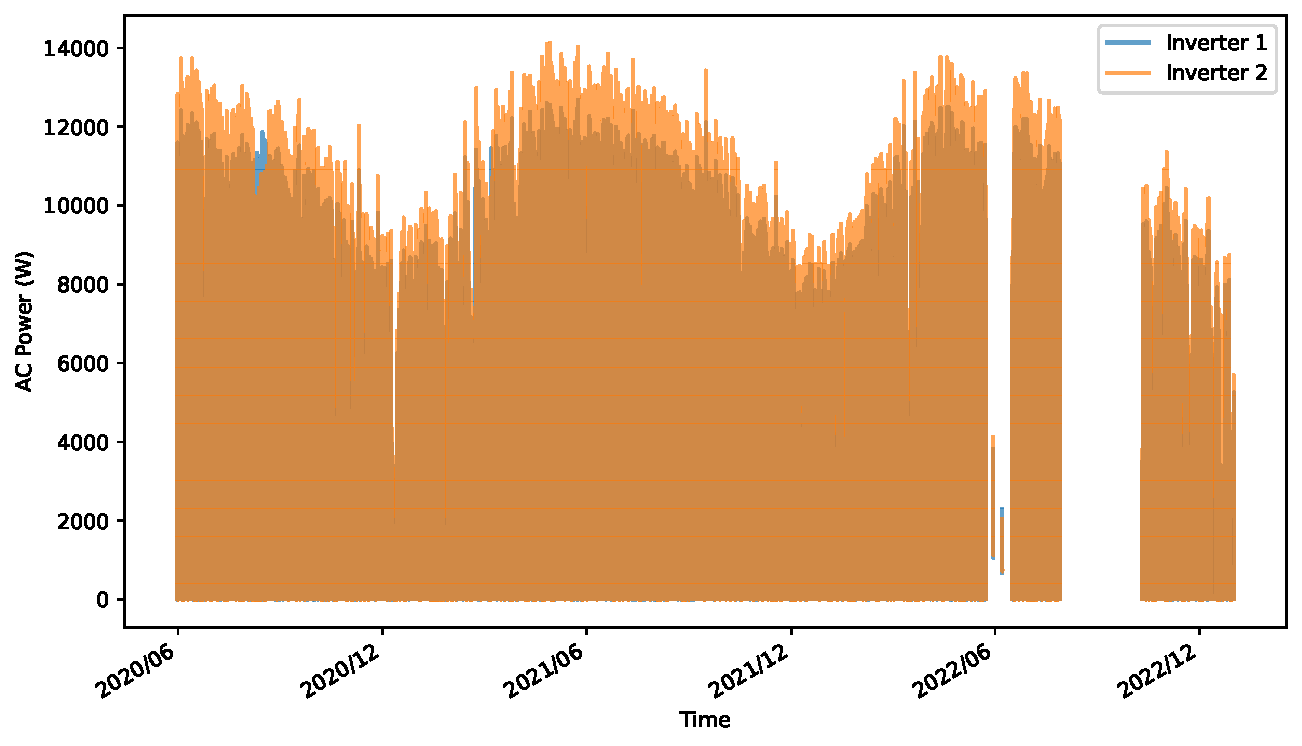
\includegraphics[width=\textwidth]{figures/chapter5/analysis/00_power_kb.pdf}
    \caption{Inverter AC side power from 2020 to 2022, used for the knowledge base.}
    \label{fig:eda_power_kb}
\end{figure}

Figure \ref{fig:eda_power_kb} shows the power profile of the two studied inverters. Right away, we notice that the power of inverter two caps at around 14kW, while inverter one usually maxes at 12kW. This information is coherent with their ratings. We can notice two relatively large chunks of missing data, with the gaps occurring in mid to late 2022.

\begin{figure}[h!]
    \centering
    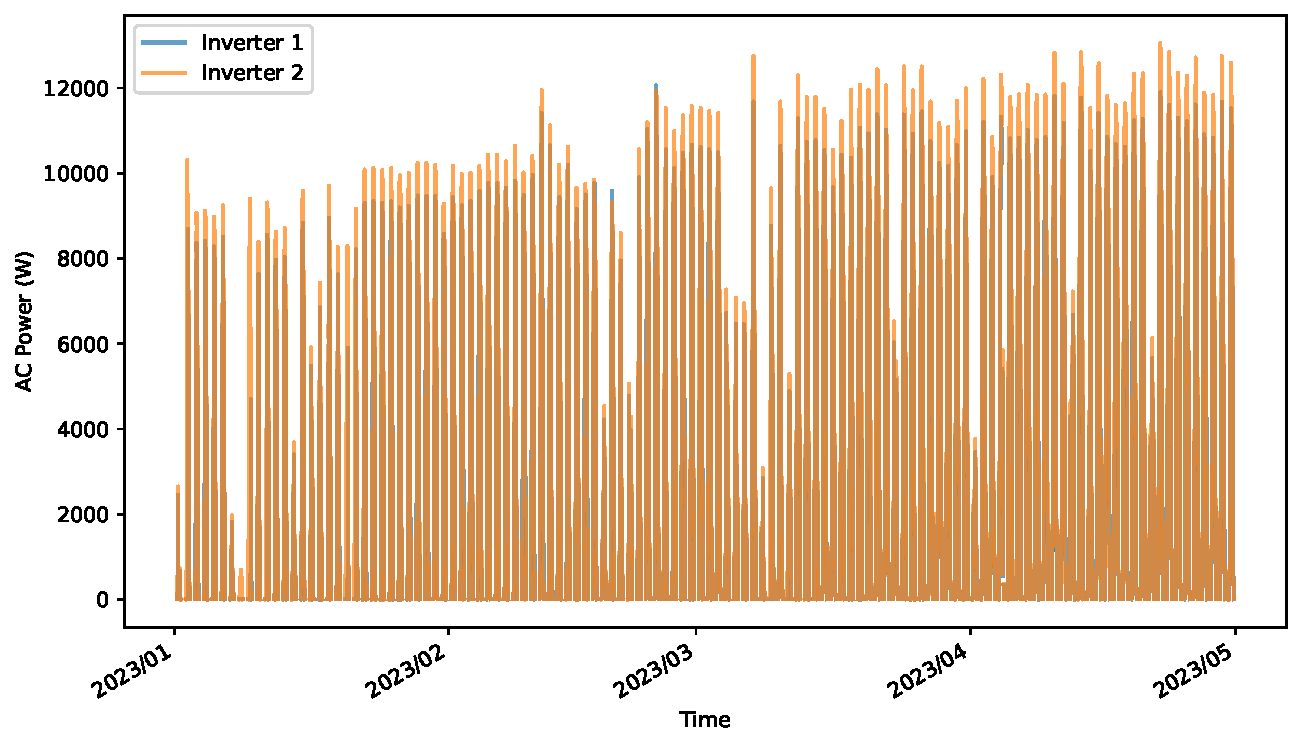
\includegraphics[width=\textwidth]{figures/chapter5/analysis/01_power_test.pdf}
    \caption{Inverter AC side power from 2023-01-01 to 2023-01-05, used for testing.}
    \label{fig:eda_power_test}
\end{figure}

Figure \ref{fig:eda_power_test} represents the power profile on the portion of data used for testing. When performing a closer inspection (with more zoom), we could hand-pick some fault occurrences in both datasets, with the majority being one inverter off while the other continues regular operation. However, these will be more noticeable during different types of data analysis, such as pair plotting. Regardless, the cases that will matter are in the test data since these scenarios will not exist in the knowledge after cleaning. In Section \ref{subsec:results}, you will find a selection of carefully chosen scenarios.

\begin{figure}[h!]
    \centering
    \includegraphics[width=\textwidth,trim={0 5.5cm 0cm 5.5cm},clip]{figures/chapter5/analysis/02_power_pairplots_kb_annotated.pdf}
    \caption{Pair plot of AC power from both inverters (2020 to 2022), using scatter (left) and KDE (Kernel Density Estimation) (right).}
    \label{fig:eda_power_kb_pair}
\end{figure}

Figure \ref{fig:eda_power_kb_pair} lets us better understand the relationship between the two inverters. As expected, since they are neighboring, this data presents a strong trend line, loading to a high Pearson coefficient: 0.97753. However, the noise from outliers is noticeable in the scatter. We define Zone A as the zone where inverter two underperforms compared to one and Zone B as the opposite. The black arrows \textcircled{\raisebox{-0.9pt}{1}} in the graph display secondary trend lines, indicating scenarios of inverter one performing consistently less than expected. Another arrow \textcircled{\raisebox{-0.9pt}{2}} also points out a cloud in Zone A (right under the trend line) of the opposite scenario. Furthermore, the red rectangles \textcircled{\raisebox{-0.9pt}{3}}\textcircled{\raisebox{-0.9pt}{4}} highlight instances where one inverter was functioning while the other was not. CellTAN must flag these situations, so we should remove them from the knowledge base. The KDE visualization confirms that most samples lie close to the primary trend.

\begin{figure}[h!]
    \centering
    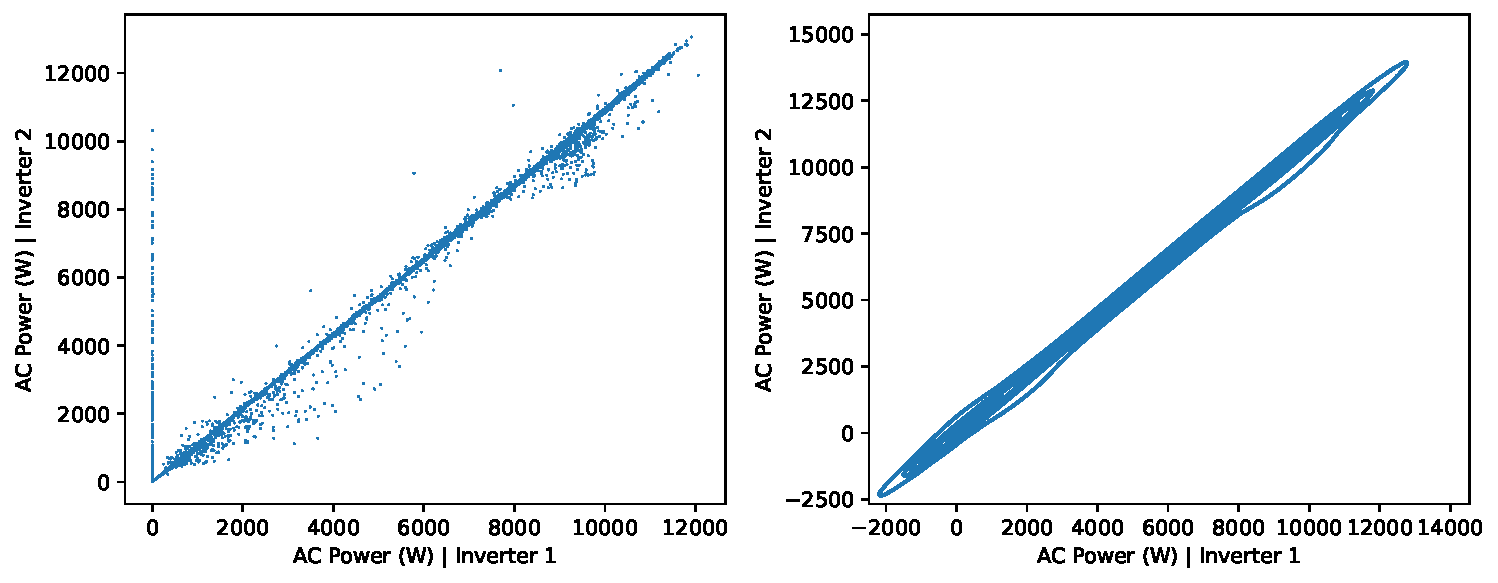
\includegraphics[width=\textwidth]{figures/chapter5/analysis/03_power_pairplots_test.pdf}
    \caption{Pair plot of AC power from both inverters (2023), using scatter (left) and KDE (Kernel Density Estimation) (right).}
    \label{fig:eda_power_test_pair}
\end{figure}

From \ref{fig:eda_power_test_pair}, it is clear that test data has fewer outliers than the previous. Nonetheless, there are many occurrences of inverter one being inoperational. Besides, there are also a considerable amount of samples below the trend line, meaning the underperformance of inverter two.

\subsubsection{Voltage and Current} \label{subsubsec:eda_volt_curr}

Both inverters are equipped with MPPTs to maximize the power output from their strings. As a result of this power converter, the current and voltage readings should fall within the optimal range of the I-V (current and voltage) curve.

\begin{figure}[h!]
    \centering
    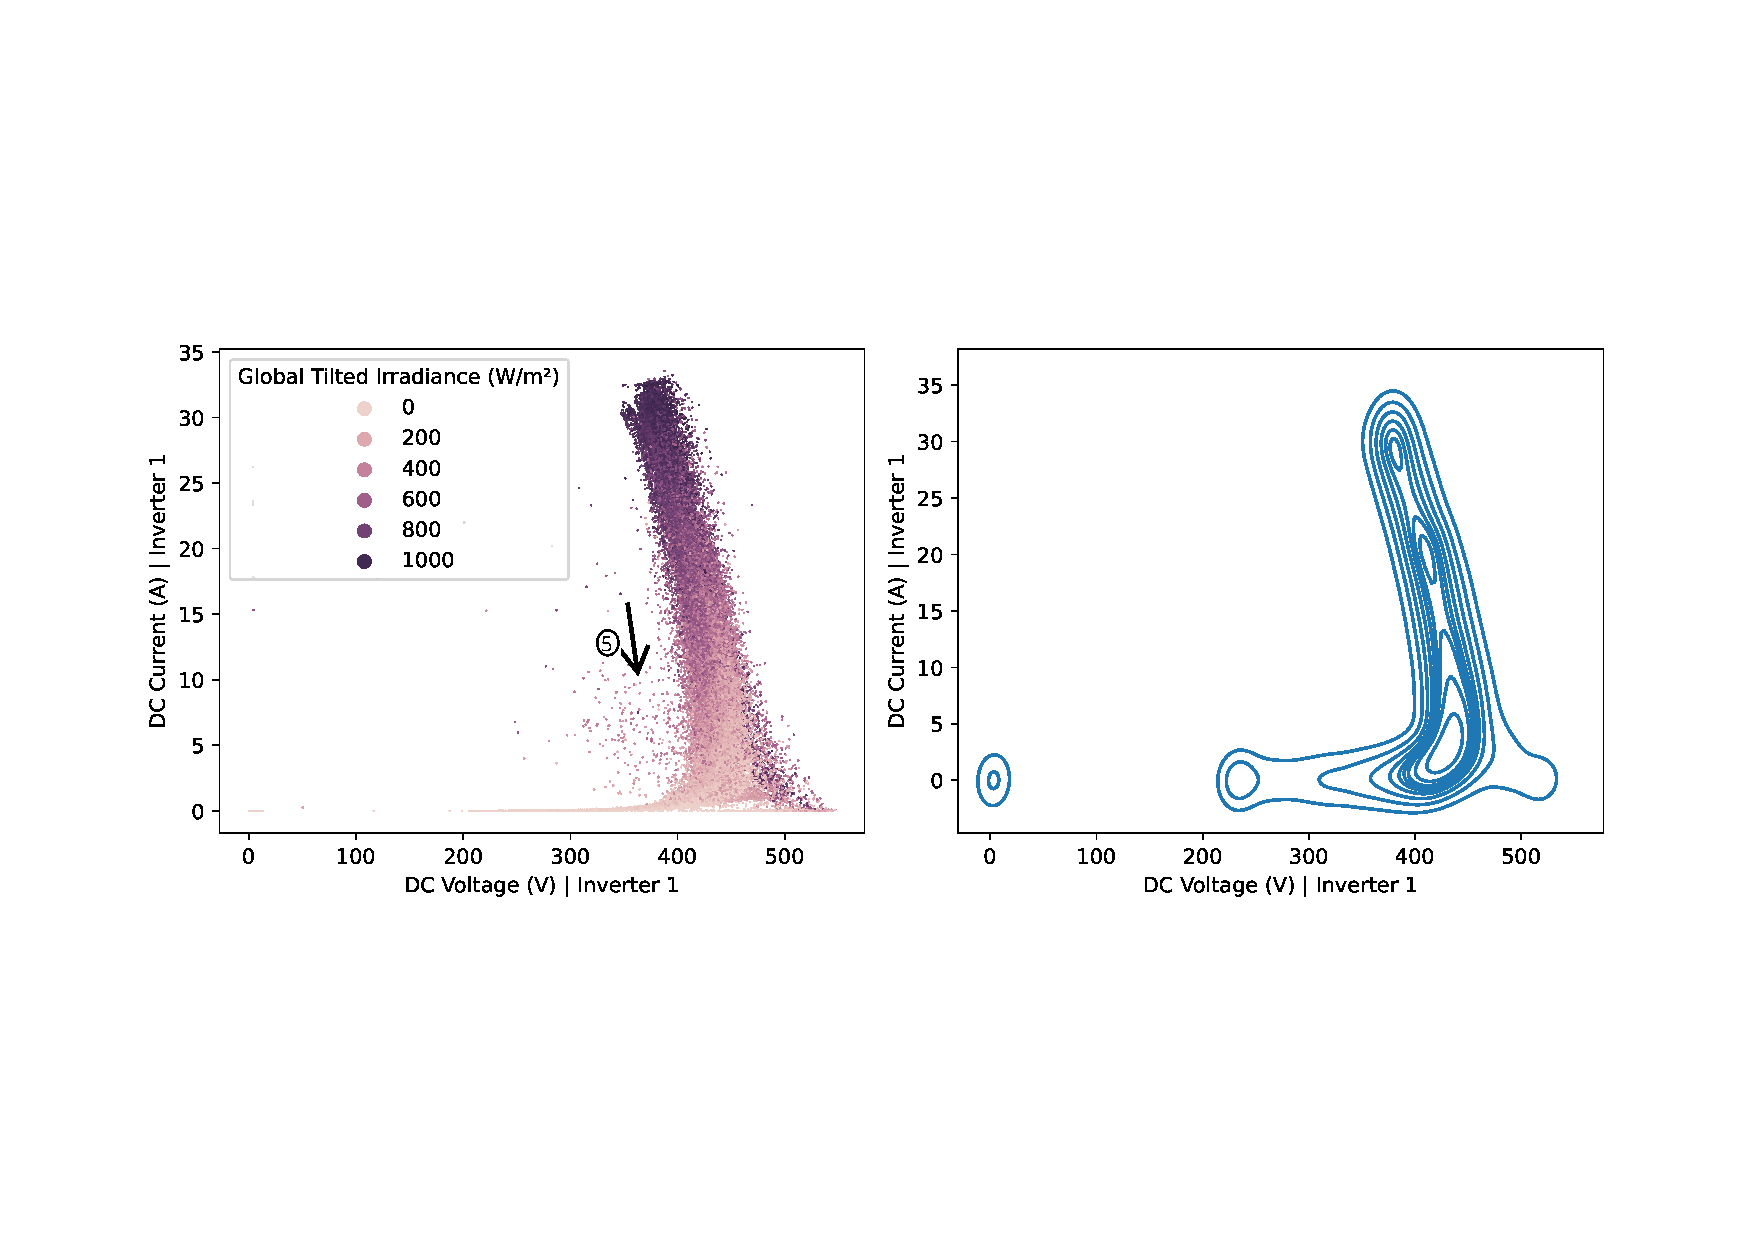
\includegraphics[width=\textwidth,trim={0 5.5cm 0cm 5.5cm},clip]{figures/chapter5/analysis/04_voltage_current_pairplot_kb_1_annotated.pdf}
    \caption{Pair plot of DC side voltage and current from inverter one (2020-2022), using scatter (left) and KDE (Kernel Density Estimation) (right).}
    \label{fig:eda_volt_curr_pair_kb_1}
\end{figure}

\begin{figure}[h!]
    \centering
    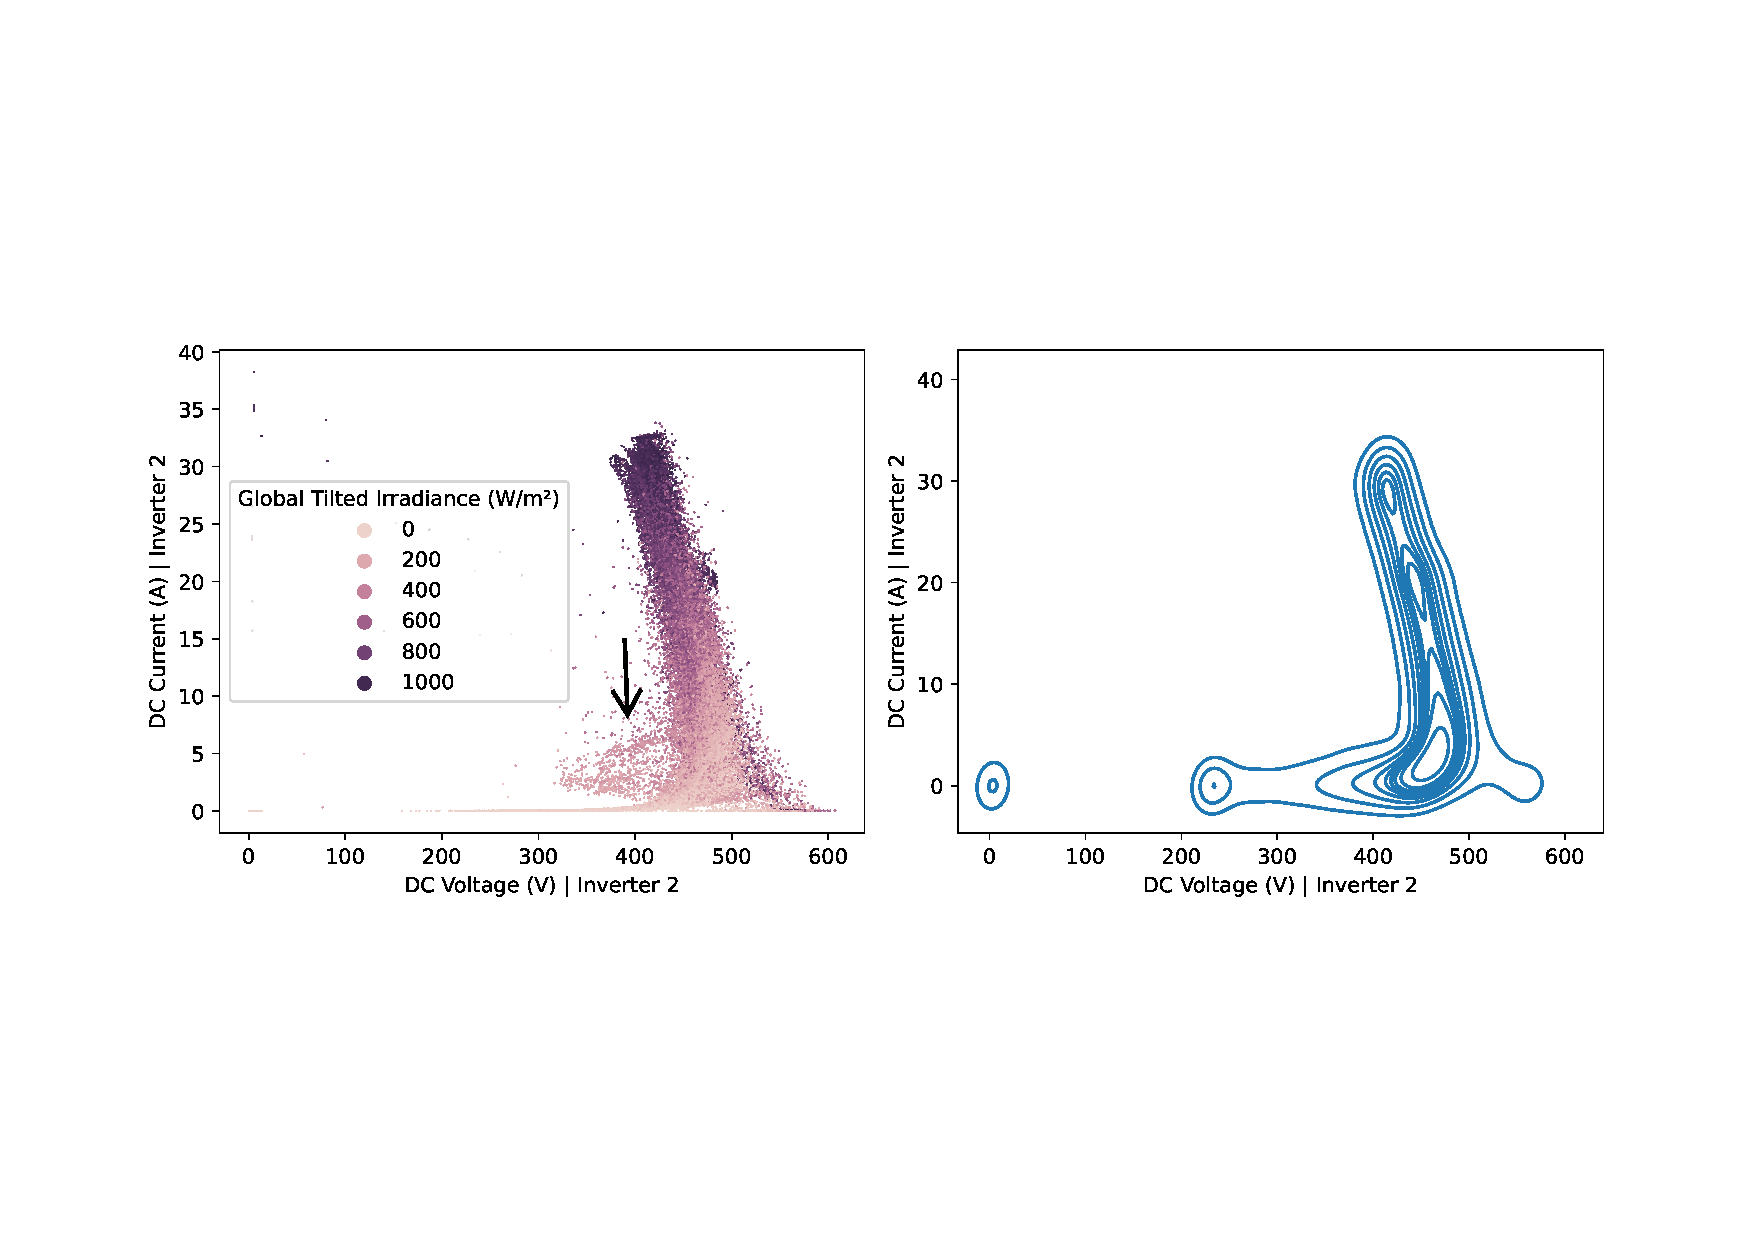
\includegraphics[width=\textwidth,trim={0 5.5cm 0cm 5.5cm},clip]{figures/chapter5/analysis/06_voltage_current_pairplot_kb_2_annotated.pdf}
    \caption{Pair plot of DC side voltage and current from inverter two (2020-2022), using scatter (left) and KDE (Kernel Density Estimation) (right).}
    \label{fig:eda_volt_curr_pair_kb_2}
\end{figure}

Regarding DC side voltage and current, figures \ref{fig:eda_volt_curr_pair_kb_1} and \ref{fig:eda_volt_curr_pair_kb_2} demonstrate the operating range of the inverter's MPPT. Both kickstart production at around 400 V and operate until close to 600 V. Between this range, the central column of samples represents voltage-current points relative to the knee of the strings' I-V curve (see figure \ref{fig:mpptcurve}), with irradiance generally increasing along its height. Some instances are outside this normal operation range (outliers), especially in the zone marked by the black arrow \textcircled{\raisebox{-0.9pt}{5}}\textcircled{\raisebox{-0.9pt}{6}}. These zones are critical because they represent inverter underperformance scenarios, which could be associated with some faults. It is denser in figure \ref{fig:eda_volt_curr_pair_kb_2}, meaning that inverter two has more underperforming situations; this was not completely clear from the previous analysis (figure \ref{fig:eda_power_kb_pair}). Appendix \ref{ap2:eda} presents the same charts, but for test data (figures \ref{fig:eda_voltage_current_test_1} and \ref{fig:eda_voltage_current_test_2}).

\subsubsection{Satellite} \label{subsubsec:eda_sat}

Irradiance should be the satellite variable most related to inverters' power. Therefore, we scatter both tilted and horizontal irradiance against AC power from inverters one and two.

\begin{figure}[h!]
    \centering
    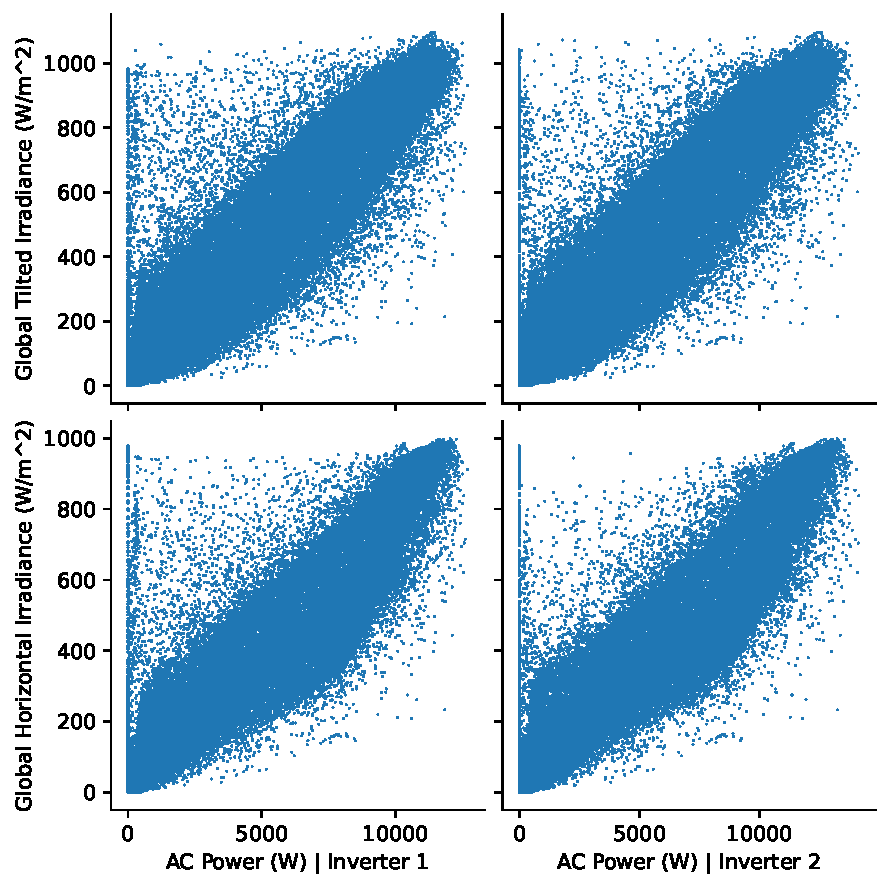
\includegraphics[width=0.8\textwidth]{figures/chapter5/analysis/08_power_irrad_pairplot_scatter_kb.pdf}
    \caption{Scatter pair plot of the AC power, tilted and horizontal global irradiance for both inverters (2020 to 2022).}
    \label{fig:eda_power_irrad_pair_kb}
\end{figure}

Figure \ref{fig:eda_power_irrad_pair_kb} shows the relationship between irradiance and AC power. We expected a positive correlation, and it exhibits such. However, the large radius around the central trend line demonstrates cycles around it that resemble some kind of hysteresis (especially with horizontal irradiance). By adding a color that displays the hour in each sample, we can affirm that these paths occur due to the fixed nature of the installed PV panels, having a characteristic curve from low to high irradiance in the sunrise and another from high to low during the sunset. Because they produce more with less sunlight in the morning, we can infer that they are oriented slightly towards the east.

Although most instances appear inside the sunrise-sunset paths, there are some outliers. The most notable are the ones of non-zero irradiance with zero production. Either error in satellite data or some anomaly in the inverters causes these odd scenarios, so we target them for cleaning the knowledge base.

Regarding the rest of the meteorological variables (cloud coverage and temperature), we deemed them unnecessary since they do not demonstrate a direct relationship with inverter behavior (see figure \ref{fig:eda_irrelevant_meteo}). We added KDE visualizations and plots for the test period in appendix \ref{ap2:eda}.

\section{Data Cleaning}

Now, we take our previous analysis and start the data-cleaning process. We used the Scikit-Learn Python Library and tried out some anomaly detection algorithms for outlier identification on our dataset: Robust Covariance \cite{Rousseeuw1999}, Isolation Forest \cite{Liu2008} \cite{Liu2012}, and Local Outlier Factor \cite{Breunig2000}. The code used for our plotting derived from an example made by Alexandre Gramfort, available on the Scikit-Learn website \cite{sklearn_example}.

\subsubsection{Power}

Based on the geographical proximity of the inverters, we have determined that the area around the trendline shown in figure \ref{fig:eda_power_kb} indicates standard operating points. Therefore, we must remove any samples deviating from this reference to clean the knowledge base.

\begin{figure}[h!]
    \centering
    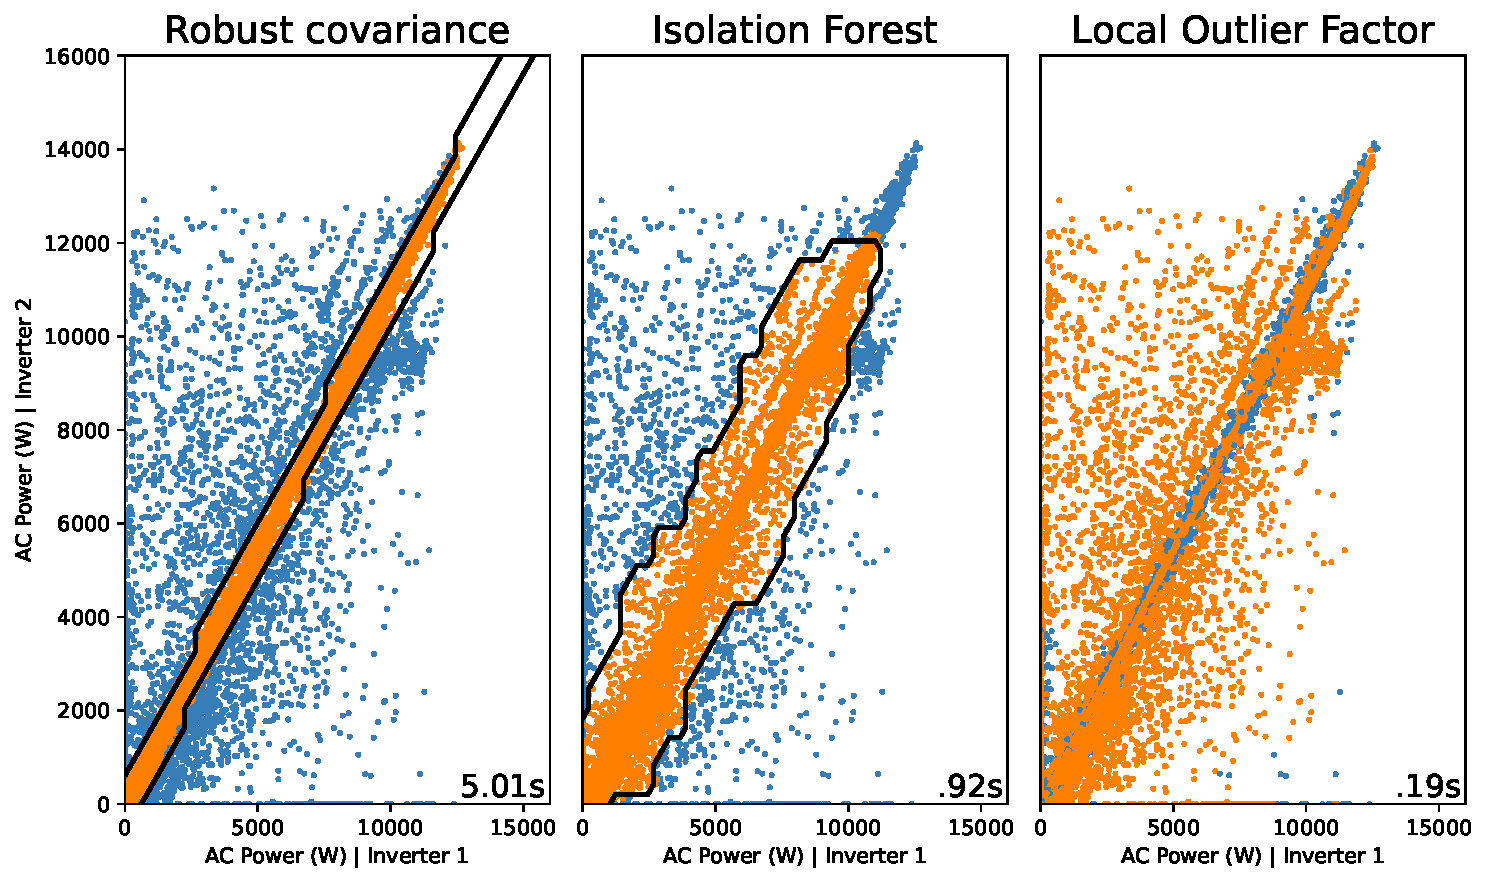
\includegraphics[width=\textwidth]{figures/chapter5/cleaning/20_cleaning_power.pdf}
    \caption{Inliers (orange), outliers (blue), and decision boundaries (black) using three different anomaly detection algorithms on the AC Power from both inverters.}
    \label{fig:clean_power}
\end{figure}

In Figure \ref{fig:clean_power}, we can see a visual representation of various anomaly detection algorithms' inliers, outliers, decision boundaries, and their computation time (bottom right). We fine-tuned the algorithms for approximately 14\% of outlier contamination. Based on the results, we determined that the Robust Covariance algorithm was the most effective since it extracted the region around the trend line without issues. We selected it to clean our knowledge base.

\subsubsection{Satellite}

In section \ref{subsubsec:eda_sat}, we discovered that the inverters follow a standard production pattern based on the irradiance and hour of the day. The specific area within the paths is considered the central region of standard operation. To clean up the data, we will remove all other instances.

\begin{figure}[h!]
    \centering
    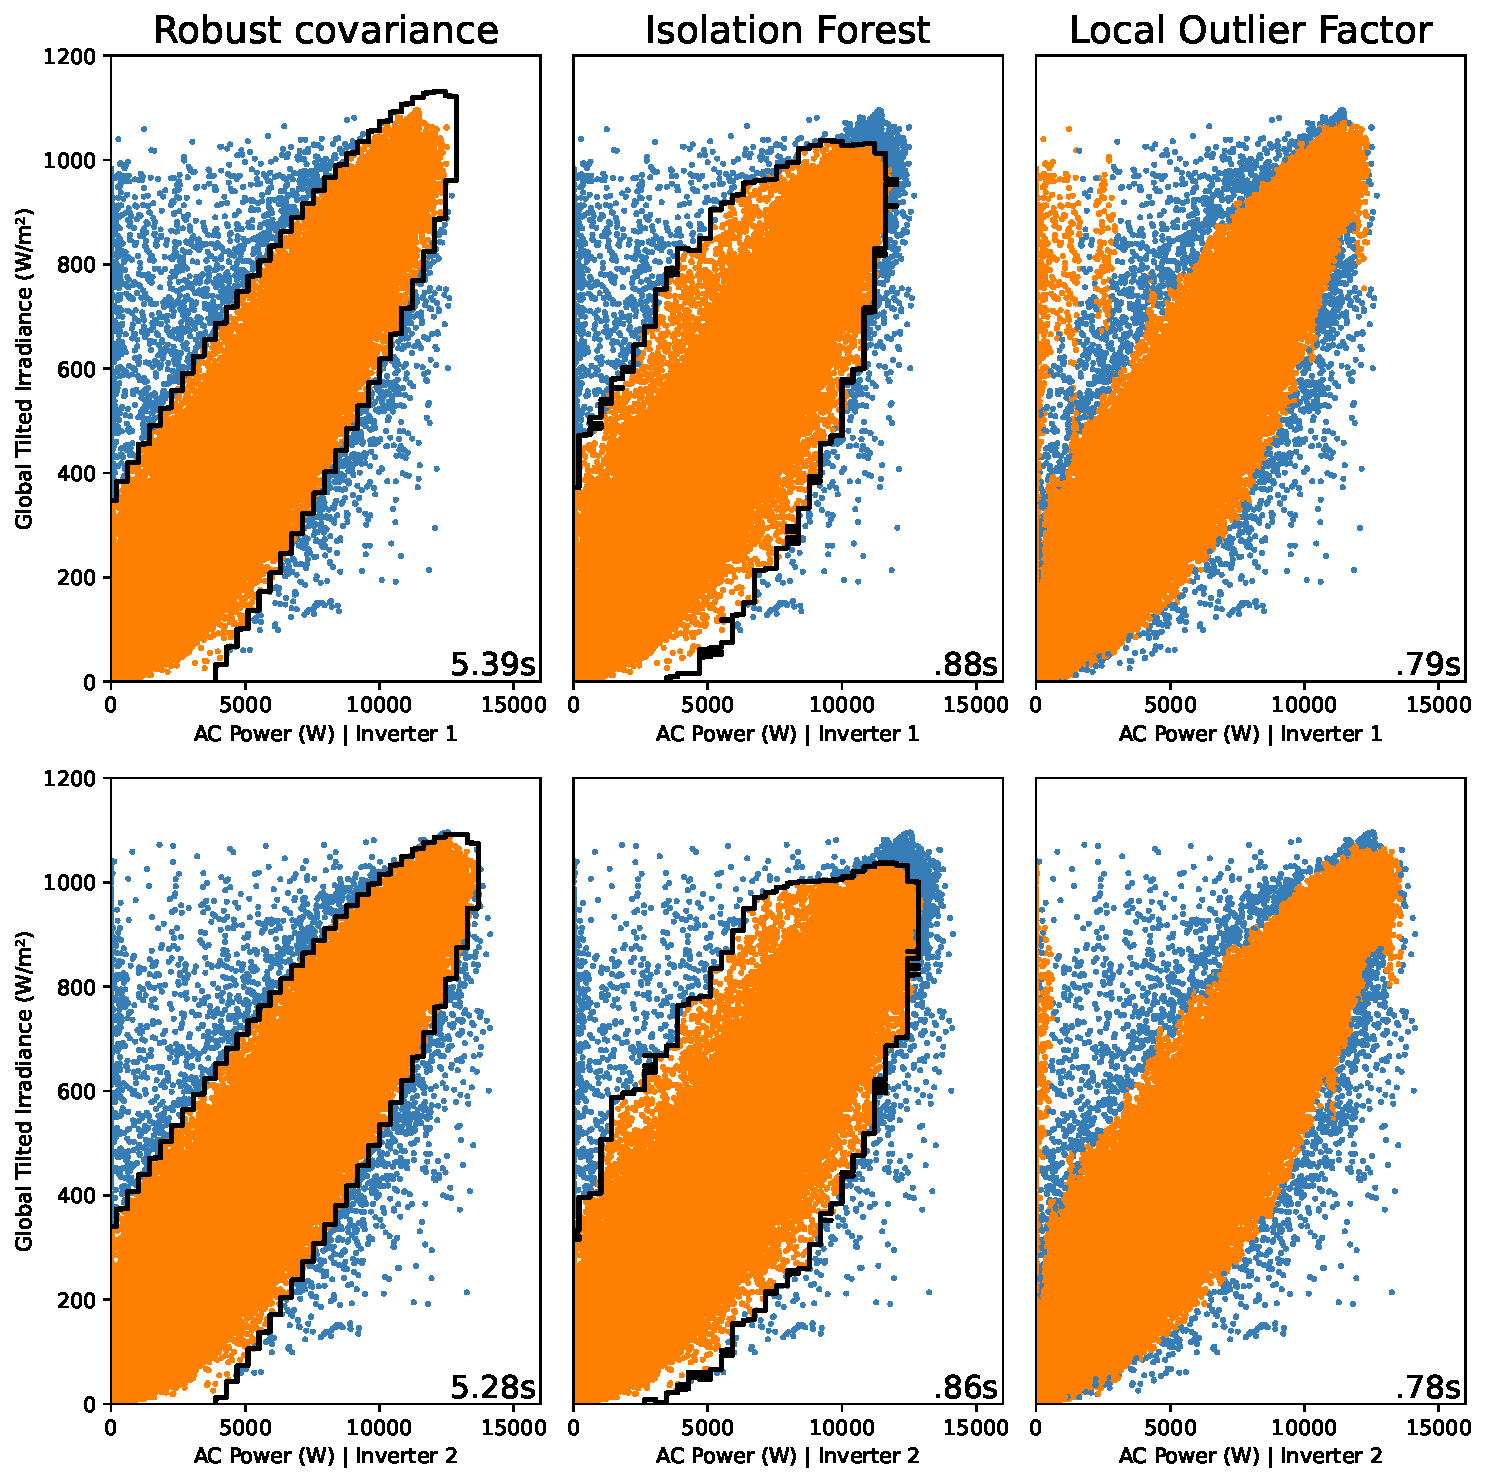
\includegraphics[width=\textwidth]{figures/chapter5/cleaning/21_cleaning_tilted_irrad.pdf}
    \caption{Inliers (orange), outliers (blue), and decision boundaries (black) using three different anomaly detection algorithms on the tilted irradiance and AC Power from both inverters.}
    \label{fig:clean_tilted_irrad}
\end{figure}

\begin{figure}[h!]
    \centering
    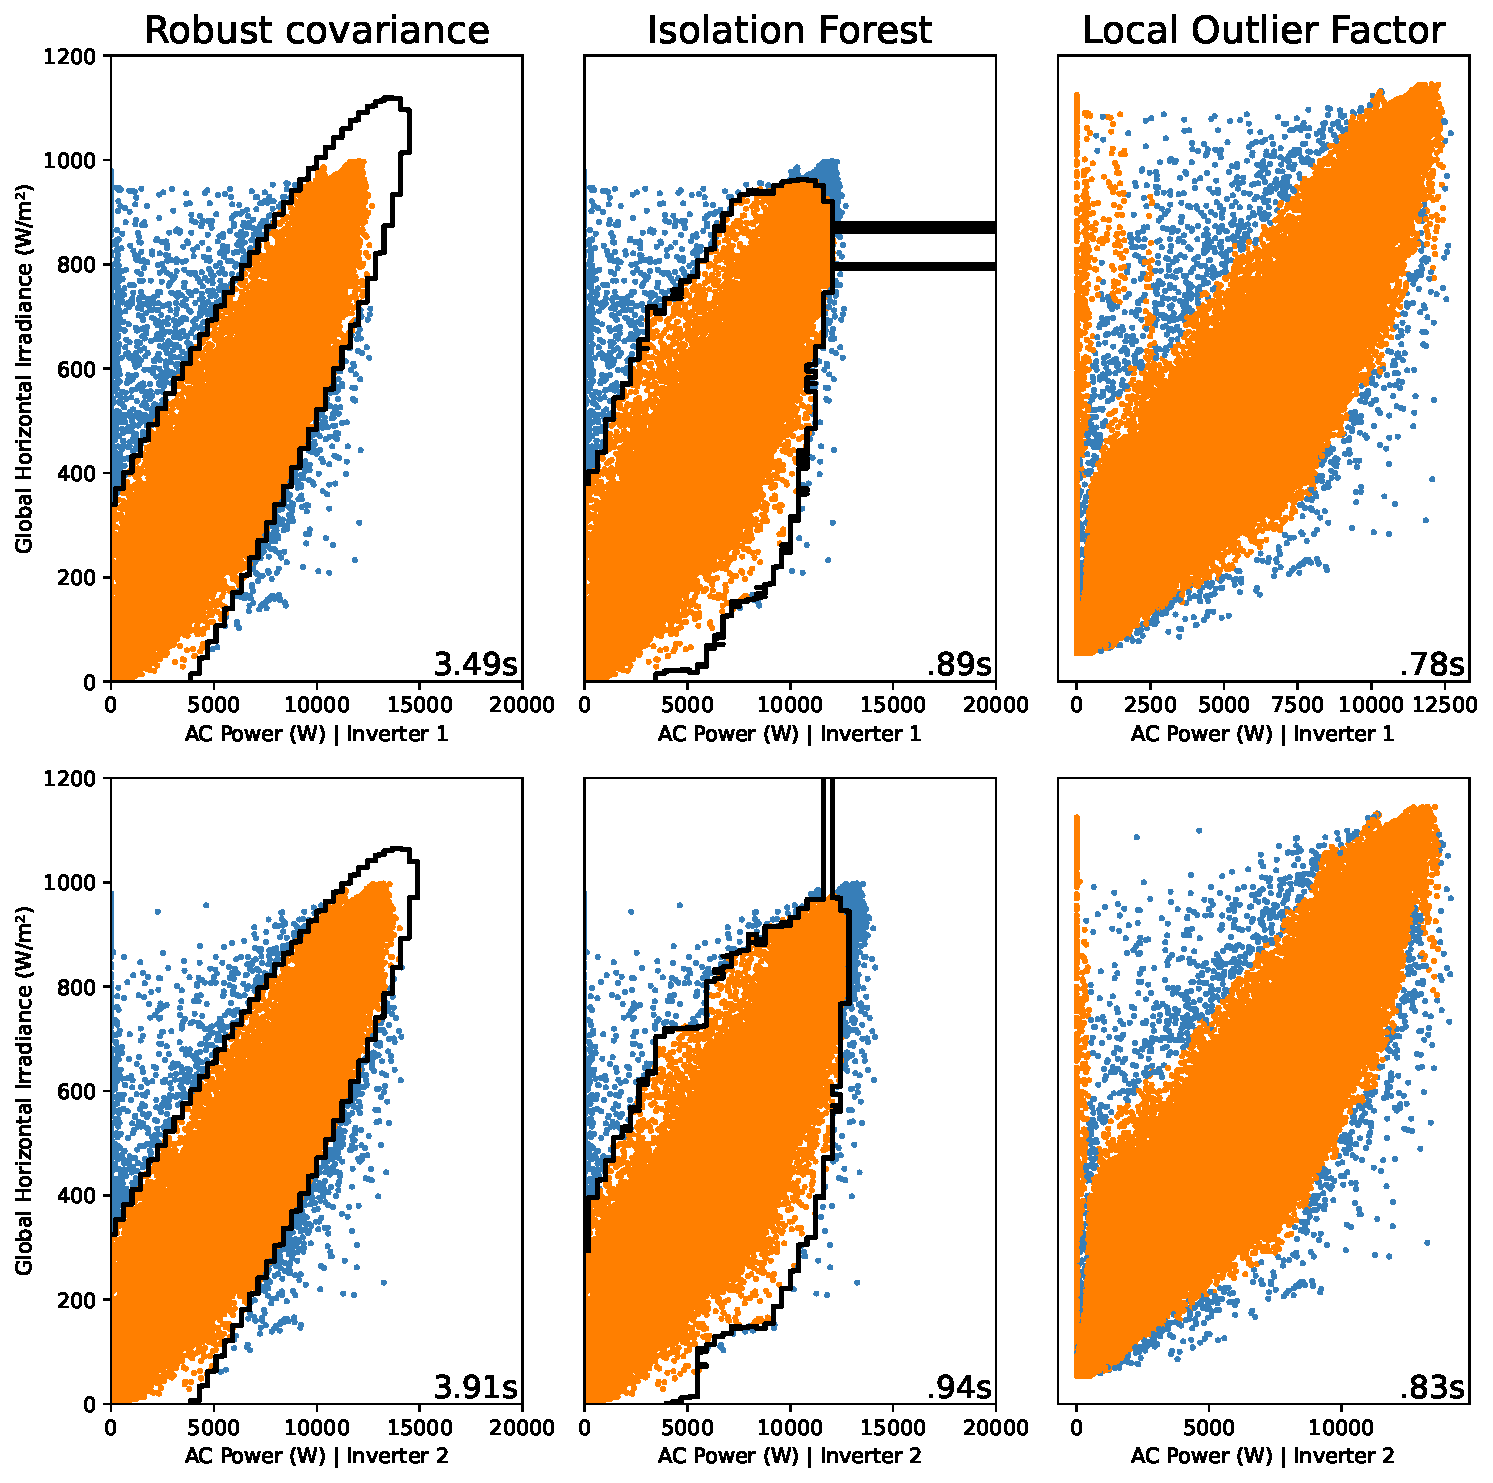
\includegraphics[width=\textwidth]{figures/chapter5/cleaning/22_cleaning_horizontal_irrad.pdf}
    \caption{Inliers (orange), outliers (blue), and decision boundaries (black) using three different anomaly detection algorithms on the horizontal irradiance and AC Power from both inverters.}
    \label{fig:clean_horizontal_irrad}
\end{figure}

Once again, figures \ref{fig:clean_tilted_irrad} and \ref{fig:clean_horizontal_irrad} demonstrate the effectiveness of the first algorithm, now for irradiance and power data. It is, once again, the chosen one for cleaning the knowledge base.

\subsubsection{Voltage and Current}

Cleaning voltage and current data were the most challenging thus far. The peculiar data distribution was an issue for all tested algorithms, and the isolation forest performed particularly poorly. We combined the Robust Covariance, and Local Outlier Factor results to obtain the best inlier-outlier separation. The aggregation performed was a logical "OR" considering the inliers.

\begin{figure}[h!]
    \centering
    \includegraphics[width=\textwidth]{figures/chapter5/cleaning/23_cleaning_volt_curr.pdf}
    \caption{Inliers (orange), outliers (blue), and decision boundaries (black) using two different anomaly detection algorithms and their combination on the DC side voltage and current from both inverters.}
    \label{fig:clean_volt_curr}
\end{figure}

The charts in figure \ref{fig:clean_volt_curr} illustrates how the algorithms have difficulty keeping up with the data's distribution and preserving the densely populated areas. Neither algorithm effectively identifies the outliers separately, but their combination proved much more effective.

\section{Photovoltaic Plugin} \label{sec:pvplugin}

According to the CellTAN formulation, cells cannot share their variables' data directly to maintain privacy. As a result, this limits plugins to work with only the information available in the cell they are running in. Therefore, inverter underperformance is the only situation considered for the PV plugin, based on the analysis from section \ref{subsubsec:eda_volt_curr}. Access to both the inverter's data and satellite data allows the owner to employ other algorithms that leverage this knowledge for better situational and fault discernment, but this falls back to the "classical" centralized algorithms, which is not the scope of this work.

We use the current and voltage samples resulting from the cleaning process to define the minimum operational boundary. Figure \ref{fig:pluginsteps} shows the proposed algorithm, which consists of the following steps:

\begin{itemize}
	\item Clean I-V data;
	\item Find the boundary points corresponding to the lowest voltage in the entire operating range;
	\item Fit a logarithmic function (\ref{eq:decayinglog}) to these points;
	\item Consider all points below the curve as situations of inverter underperformance.
\end{itemize}


Since data cleaning is already covered, we describe ways of determining the boundary points.
To begin, we establish bins for the current samples with a size of 1 A. Next, we examine each bin and determine the minimum voltage for that particular region via either the absolute minimum or a quantile. Once we have selected the reference minimum voltage, we record the bin's median current and minimum voltage as a boundary point.
After registering all boundary points, we use a curve-fitting algorithm to apply a decaying logarithmic function to them (equation \ref{eq:decayinglog}).

\begin{equation} \label{eq:decayinglog}
    V = a \times log(b \times I + c) + d \times I + e 
\end{equation}
where:
\begin{align*}
    V & : \text{Voltage (V)} \\
    I & : \text{Current (A)} \\
    a,b,c,d,e & : \text{Unknown constant parameters}
\end{align*}

\begin{figure}[h!]
    \centering
    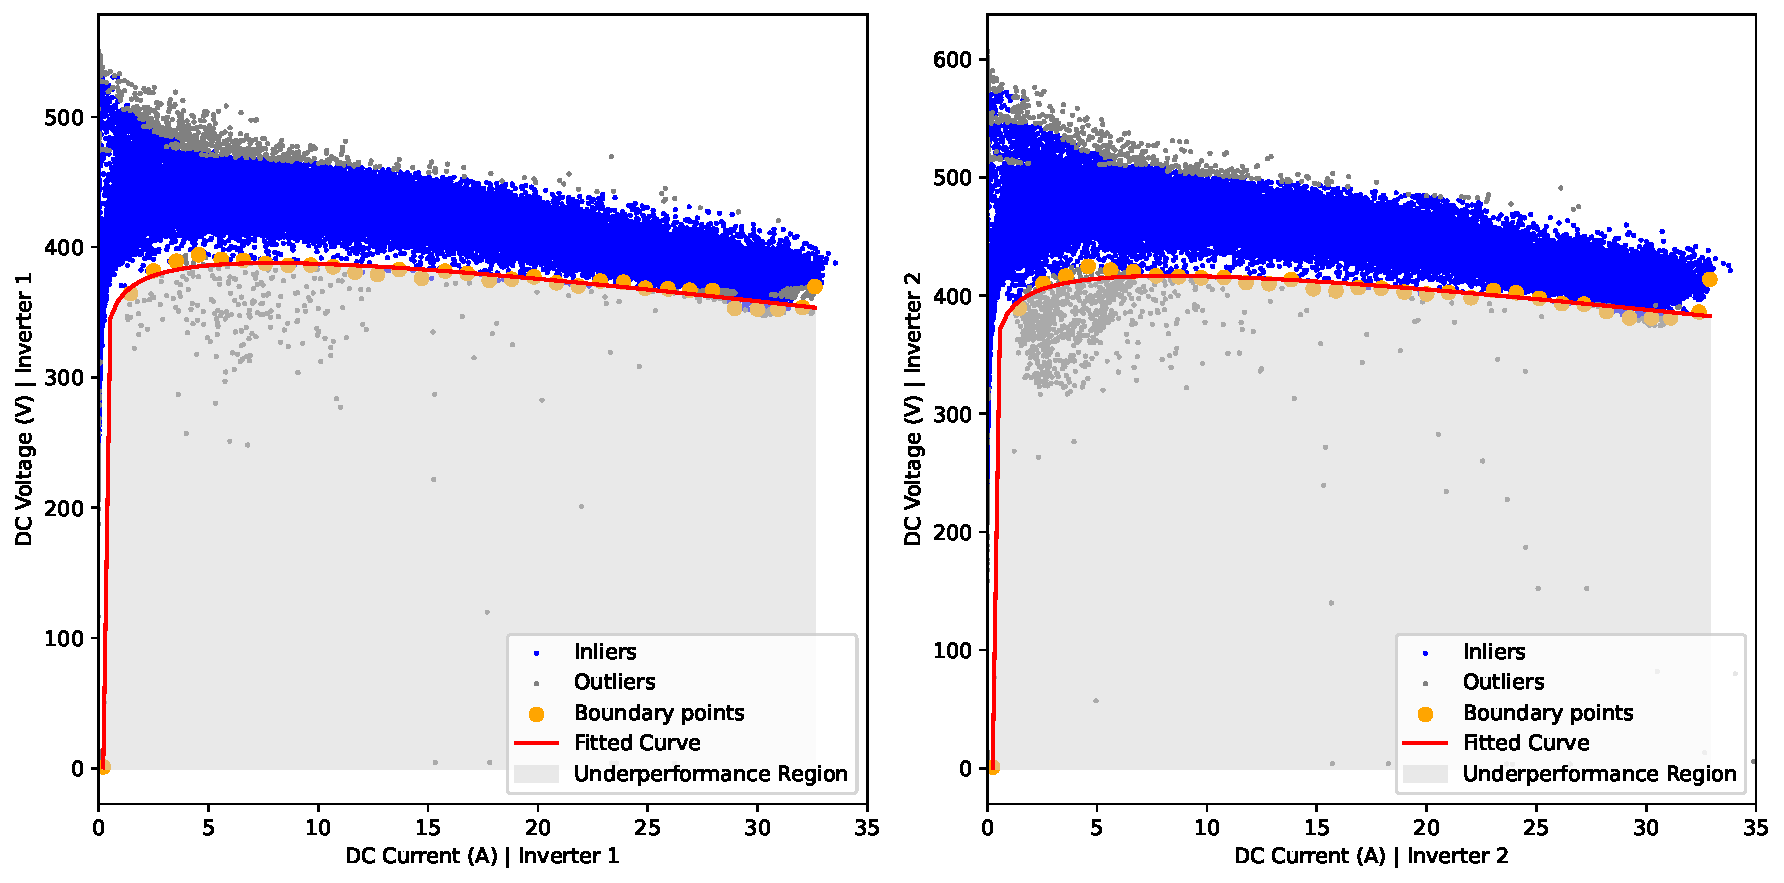
\includegraphics[width=\textwidth]{figures/chapter5/algorithm/30_boundary.pdf}
    \caption{Inverter underperformance region based on the lowest boundary of current-voltage inliers.}
    \label{fig:anomaly_decision_boundary}
\end{figure}

Figure \ref{fig:anomaly_decision_boundary} illustrates the outcome of using the described algorithm on our case study inverters. With the fitted curve's parameters, the PV plugin can analyze a new sample and determine if it falls under the underperformance category—whenever it does, the plugin flags that situation and reports back to the cell.
The fitted logarithmic curves are:

$$
    V_{inverter1} = 19.3 \times ln(169.2 \times I_{inverter1} - 35.2) - 2.8 \times I_{inverter1} + 276.1
$$

$$
    V_{inverter2} = 20.6 \times ln(148.3 \times I_{inverter2} - 35.6) - 2.9 \times I_{inverter2} + 299.5 
$$

\section{CellTAN Configuration}

Implementing CellTAN for cells running online requires significant time and resources to gather meaningful results. Therefore, we created a virtual scenario to simulate test data and collect outputs quickly. The simulation involves cells using fake in-memory implementation of some of their dependencies, such as the interface and repository. The interface serves for cell communication, and the in-memory implementation allows cells in the same host to share information without the overhead of a communication protocol. The repository is where the cell keeps its knowledge base and other persisted attributes (e.g. trust with neighbors). An in-memory implementation eliminates the need to set up a database for experimentation, speeding up data lookup and storage.

To maintain time fidelity, the most crucial requirement of this tool, we have the cells use a custom rolling timestamp generator that follows the time of each sample passed to the inputs. In practice, we "tell" the cells what time it is instead of them recurring to the standard date-time library. This workaround effectively makes all the mechanisms of the cell function without direct modification: their current time is always correct relative to the inputs. This workaround allows feeding cells new inputs as fast as they perform their main process loop, which was one of the most impactful changes for simulation speed.

Selecting cell parameters can be difficult due to the complexness of variable uncertainties and thresholds (\ref{subsec:cellconfig}). However, besides variables' uncertainty and bounds, most parameters are subjective to the intentions of a cell owner, while almost everything derives from the trust measurements. Therefore, instant trust values are a more reliable source for result analysis, compared to the subjective cell state attribute.

We selected AC power, DC side current, and voltage for the inverters' inputs, considering 5\% uncertainty on all variables. For the satellite, we used global tilted irradiance and global horizontal irradiance, also with 5\% uncertainty each. The complete cell configuration is available in appendix \ref{ap2:cellconfig}.

% ! TODO mais info aqui?

\section{Simulation and Results} \label{subsec:results}

\subsection{Artificial Network Simulation}

To validate the CellTAN core mechanisms with a controlled scenario, we simulate a network of only two cells (two inverters) with the same knowledge base (of inverter one). This way, we have a clean slate for introducing anomalies and watching the corresponding behavior. Translating to a real case, this would be most similar to two equal inverters with the same PV configuration installed in the same place.

\subsubsection{Simulation Without Anomalies}  \label{subsubsec:simnoanom}

We are conducting our initial validation using a scenario without any anomalies. To achieve this, we will simulate 73 instances of a clear day, starting from 06:30:00 on March 2nd, 2023, and ending at 18:30:00 on the same day.

\begin{figure}[h!]
    \centering
    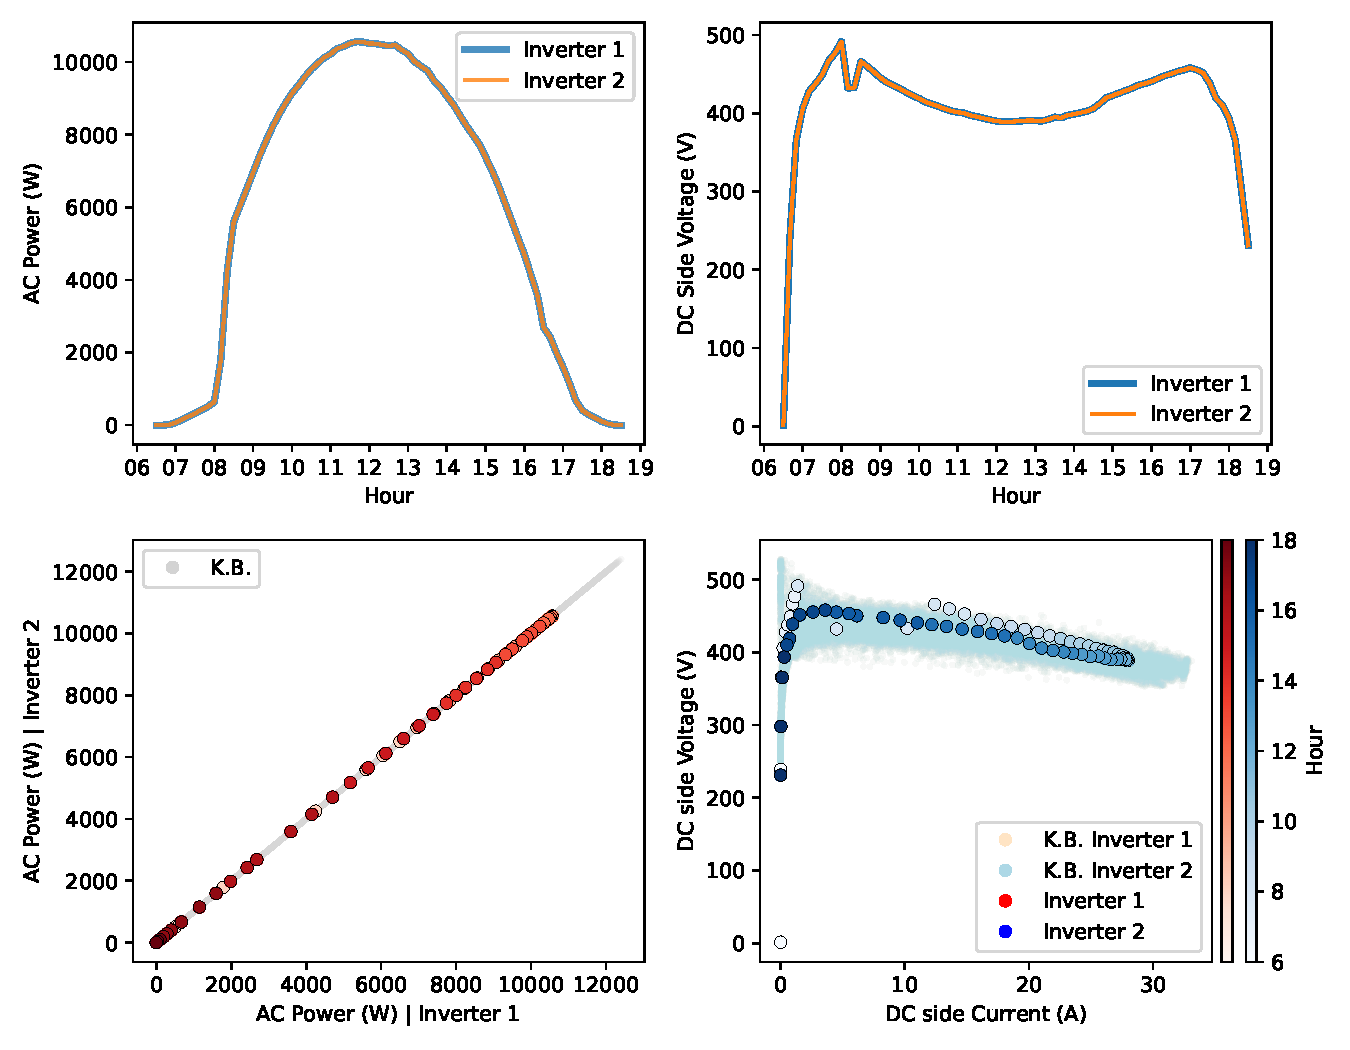
\includegraphics[width=0.9\textwidth]{figures/chapter5/results/artificial/40_test_clone_01.pdf}
    \caption{Power, current, voltage profiles, and scatter of simulation data for the artificial scenario without anomalies.}
    \label{fig:artificial_01_piv}
\end{figure}

To showcase the data received by CellTAN, we utilize visualizations such as \ref{fig:artificial_01_piv}. The term "K.B." stands for Knowledge Base, and the scatter plots help comprehend the input's space compared against it. This shows if we introduced anomalies or not.

We can see that having cloned inverters creates a perfect trend line in their AC power scatter. The voltage profile for the tested day is relatively typical, with a slight dip at around hour 8. The scatter shows that most samples lie within the knowledge base, except for some in the morning, almost exceeding the upper voltage border.
We don't expect the CellTAN to indicate any issues for this base scenario.

\begin{figure}[h!]
    \centering
    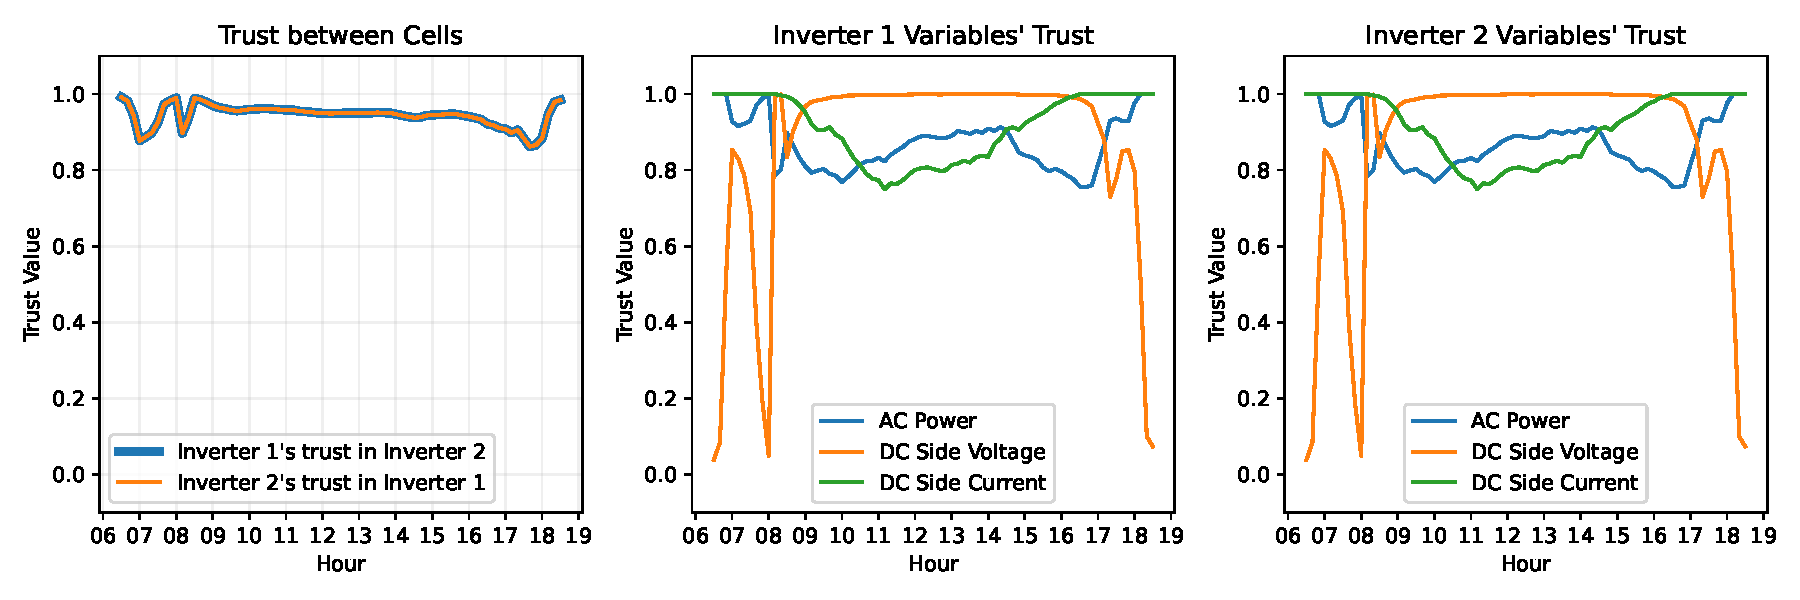
\includegraphics[width=\linewidth]{figures/chapter5/results/artificial/42_results_test_clone_01.pdf}
    \caption{Inverter's trust and variables' trust from CellTAN for the artificial scenario without anomalies.}
    \label{fig:artificial_results_01}
\end{figure}

Figure \ref{fig:artificial_results_01} shows the expectable high trust measure between inverter cells, with an average rating of 0.94. However, the variation in this rating and the fact that it falls just below 1 is due to the uncertainty involved in the trust calculation process, as highlighted in Figure \ref{fig:trust_test_3}. Based on the observed behavior, the cells have encountered numerous similar past instances. Therefore, we infer that reduced variable uncertainties (parametrized) would lead to an improved trust indicator in this context (topic developed in section \ref{subsec:trust}).


Variables' trust is relatively stable from hours 9 to 17. However, there are issues with this indicator for DC voltage during sunrise and sunset. These momentary drops occur due to the inconsistency of samples in these extremes, given that the original dataset did not store values beyond a certain threshold (considered nighttime). Voltage measurements in these zones are erratic, so a moving average is more appropriate to smooth out these trust oscillations and better assess the possibility of anomaly. We take this occurrence into account for the subsequent experiments.
With this scenario, we also check the symmetry of the trust indicator, which is identical for the pair of cells. The PV plugin did not flag any underperformance situations during this simulation, as expected.


\subsubsection{Simulation With Anomalies}

To assess the CellTAN's anomaly detection capability, we simulate inverter mismatch and underperformance for the same day as the previous experiment. We expect the perturbance to influence the cells' trust measurement into lowering and trigger the PV plugin to warn the situation.

\begin{figure}[h!]
    \centering
    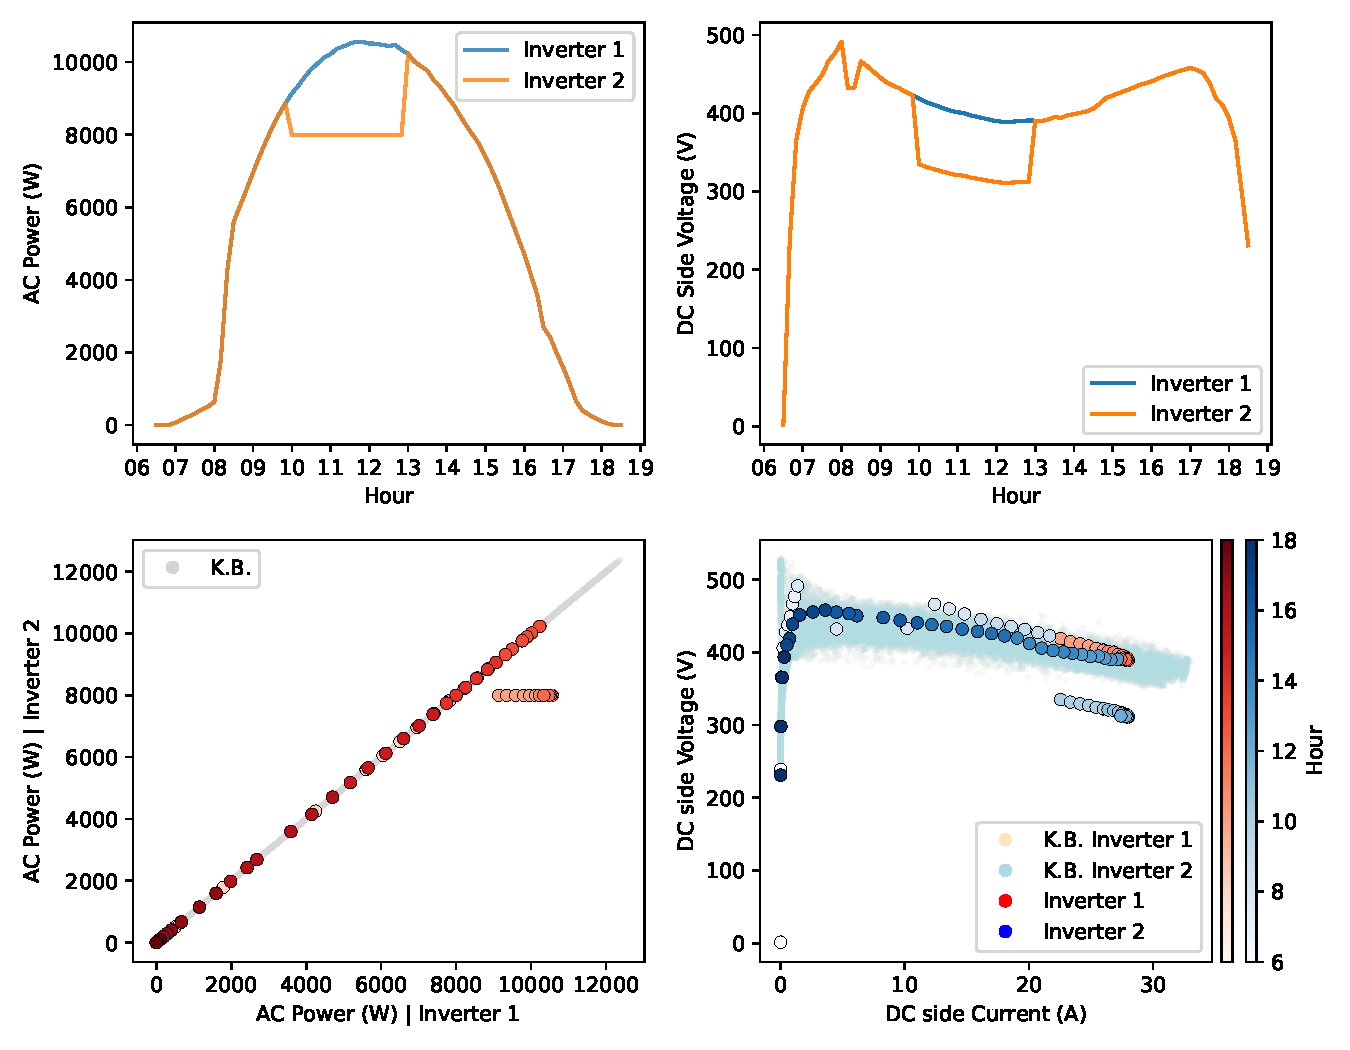
\includegraphics[width=0.9\textwidth]{figures/chapter5/results/artificial/41_test_clone_02.pdf}
    \caption{Power, current, voltage profiles, and scatter of simulation data for the artificial scenario with anomalies.}
    \label{fig:artificial_02_piv}
\end{figure}

Figure \ref{fig:artificial_02_piv} shows the artificial anomaly introduced in the AC power and DC side voltage measurements, representing the underperformance of inverter two. Regarding the AC power scatter, it resembles region \textcircled{\raisebox{-0.9pt}{2}} of figure \ref{fig:eda_power_kb_pair}. Observing the I-V scatter in the bottom right, we can also notice that the introduced anomaly translates some instances into the underperforming region, mapped in the previous section (\ref{sec:pvplugin}).
We expect CellTAN's cell trust mechanism and the PV plugin to catch this situation.

\begin{figure}[h!]
    \centering
    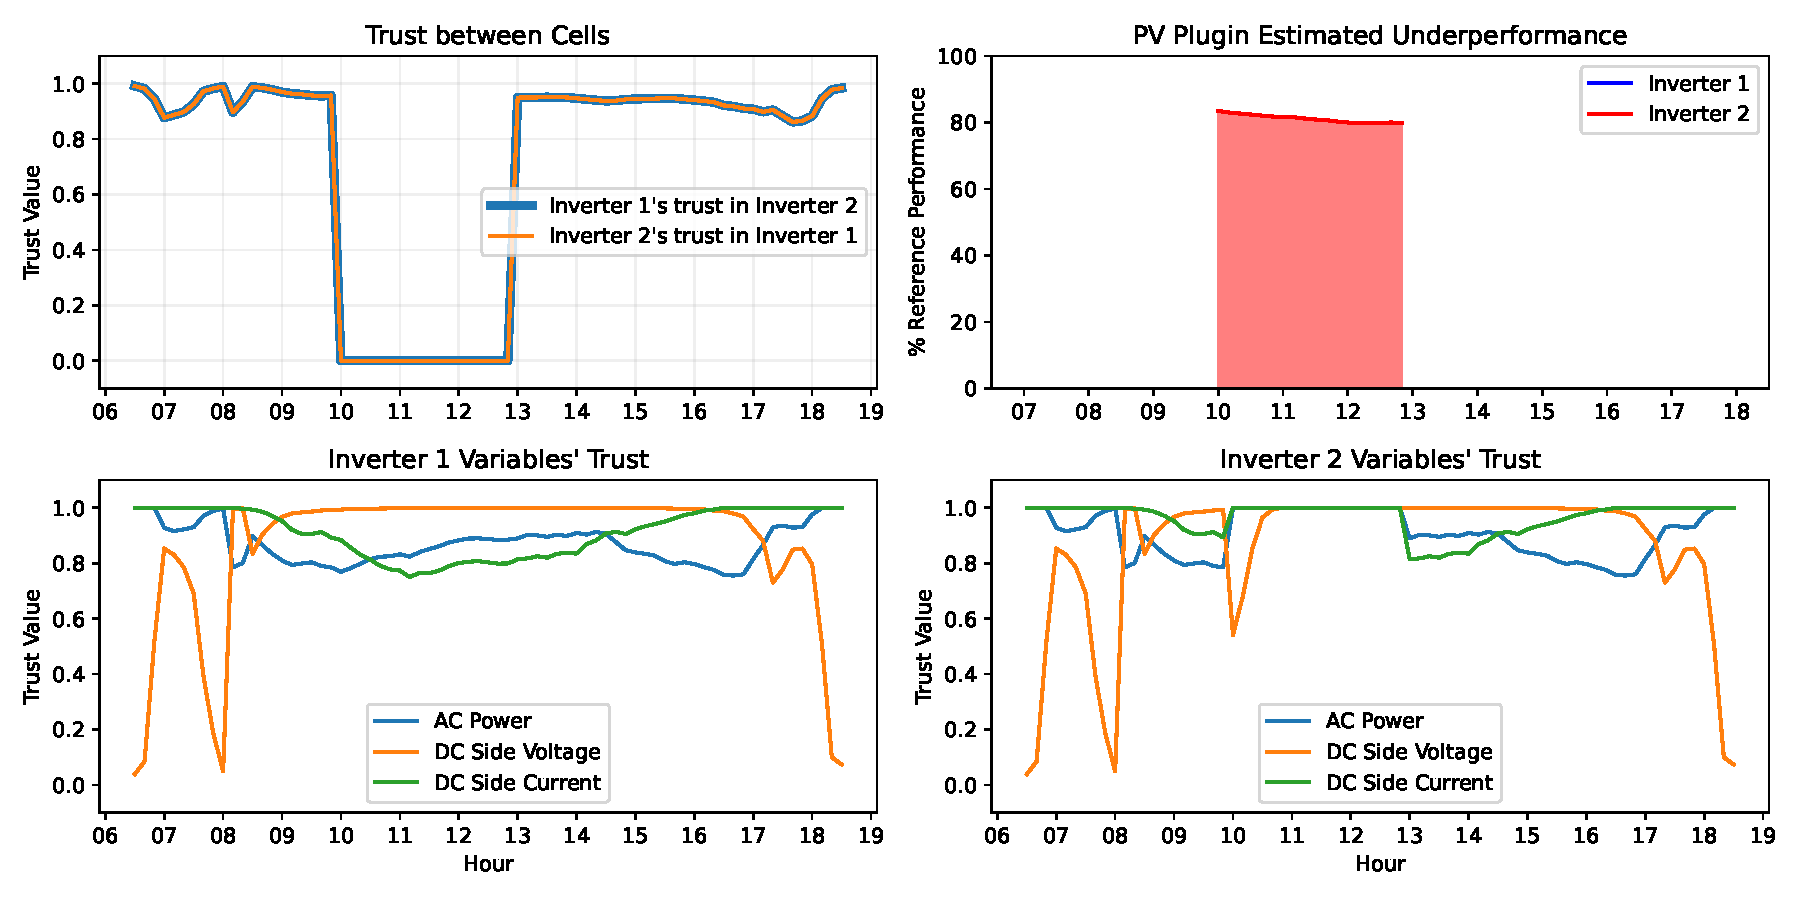
\includegraphics[width=\textwidth]{figures/chapter5/results/artificial/43_results_test_clone_02.pdf}
    \caption{Inverter's trust and variables' trust from CellTAN for the artificial scenario with anomalies.}
    \label{fig:artificial_results_02}
\end{figure}

Figure \ref{fig:artificial_results_02} shows that the trust between cells drops to (practically) zero while the anomaly occurs. This behavior perfectly aligns with the historical trust comparison process of using a moving average to consider unconformities, given a threshold. This way, if the cell owner had configured the cell to have a three-hour trust bin comparison and an appropriate threshold, this situation would be flagged at hour 13.

One major issue with the symmetry of the cell trust measure is that we need further assessment to understand which is the faulty element. Variables' trust indicators and plugins come to support this necessity. In this specific scenario, variables' trust showed a momentary drop for the DC side voltage, but not significant enough to distinguish from the ones in the sunrise and sunset transitions. However, the PV plugin flagged inverter two's underperformance, indicating the power was around 80\% of the expected minimum throughout the anomaly (figure \ref{fig:artificial_results_02}, top right chart). This indicator is enough, in this context, to distinguish which is the faulty inverter.

\subsection{Real Network Simulation}

Although artificial scenarios have their place for conceptual validation, data from a physical cell network is valuable for assessing the usefulness of our fault detection tool. In the following sections, we use the test data from both inverters and satellite reviewed in \ref{sec:case_study} to run the CellTAN.

Using four months' data allows for statistically evaluating the tool's outputs, considering it has a broad range of scenarios. However, selecting which portions of the result dataset to showcase in the following sections becomes challenging. Nevertheless, this is also needed to understand real-time behavior, so the presented results will be hand-picked sections with relevancy.

The CellTAN contains a lot of valuable attributes for assessing the cell's state, such as its variables' fuzzy outputs, cell/variables trust indicators, extrinsic/intrinsic unconformity severity (with incoherent element information), and situations detected by plugins. However, we minimize overloading our findings with all this data and focus on the most objective indicators: outputs, trust indicators, variables' inputs, and the underperformance estimation from the PV plugin. The state data and unconformity information depend on arbitrary time bins and thresholds. Since it derives from the instantaneous trust values, and the cell owner controls such parameters, we omit these state attributes (same as the artificial scenario).

\subsubsection{Trust Indicators Overview}

After gathering results, visualizing the relation between inverter trust and outlier regions defined in section \ref{subsec:eda} gives a direct view of CellTAN's anomaly detection capabilities.

\begin{figure}[h!]
    \centering
    \includegraphics[width=\textwidth]{figures/chapter5/results/real/52_scatter_with_trust.pdf}
    \caption{Scatter of inverter AC power (1st) and inverter variables (2nd and 3rd), colored with the trust value between inverters.}
    \label{fig:real_sim_trust_scatter}
\end{figure}

Figure \ref{fig:real_sim_trust_scatter} confirms that the tool consistently assigns low trust values to instances in outlier regions, denoted by the darker tone. We expected the performance to be satisfactory since the cells' knowledge base went through a cleaning phase, making the temporal similarity extraction process and cell activations prone to mainly capture what we predefined as correct behavior.

Regarding the distribution of trust indicators in figure \ref{fig:cell_trust_hist}, the measure between inverters shows that most instances have high values, with the majority above 0.7. These histograms do not include samples at night since all the outputs remained constant. The first bin on the left chart of \ref{fig:cell_trust_hist}, which contains values close to zero, is the most significant region for determining anomalies when using the trust of inverter cells. Considering this bin, we may establish that around 500 samples are anomalous out of the 4464 (11.2\%).

Unfortunately, the distributions of trust between inverters and satellite indicate that these connections did not benefit the tool. These results suggest that the trust calculation system is less versatile than foreseen and requires modification for leveraging these cell links. Earlier, we aligned the uncertainty of the satellite variables with that of the inverters while configuring the cells, hoping to match their time similarity extraction. However, remembering the trust calculation method, we conclude that systems can have different time extraction characteristics, leading to lower trust when this leads to significant differences in the cells' total activation time.

\begin{figure}[h!]
    \centering
    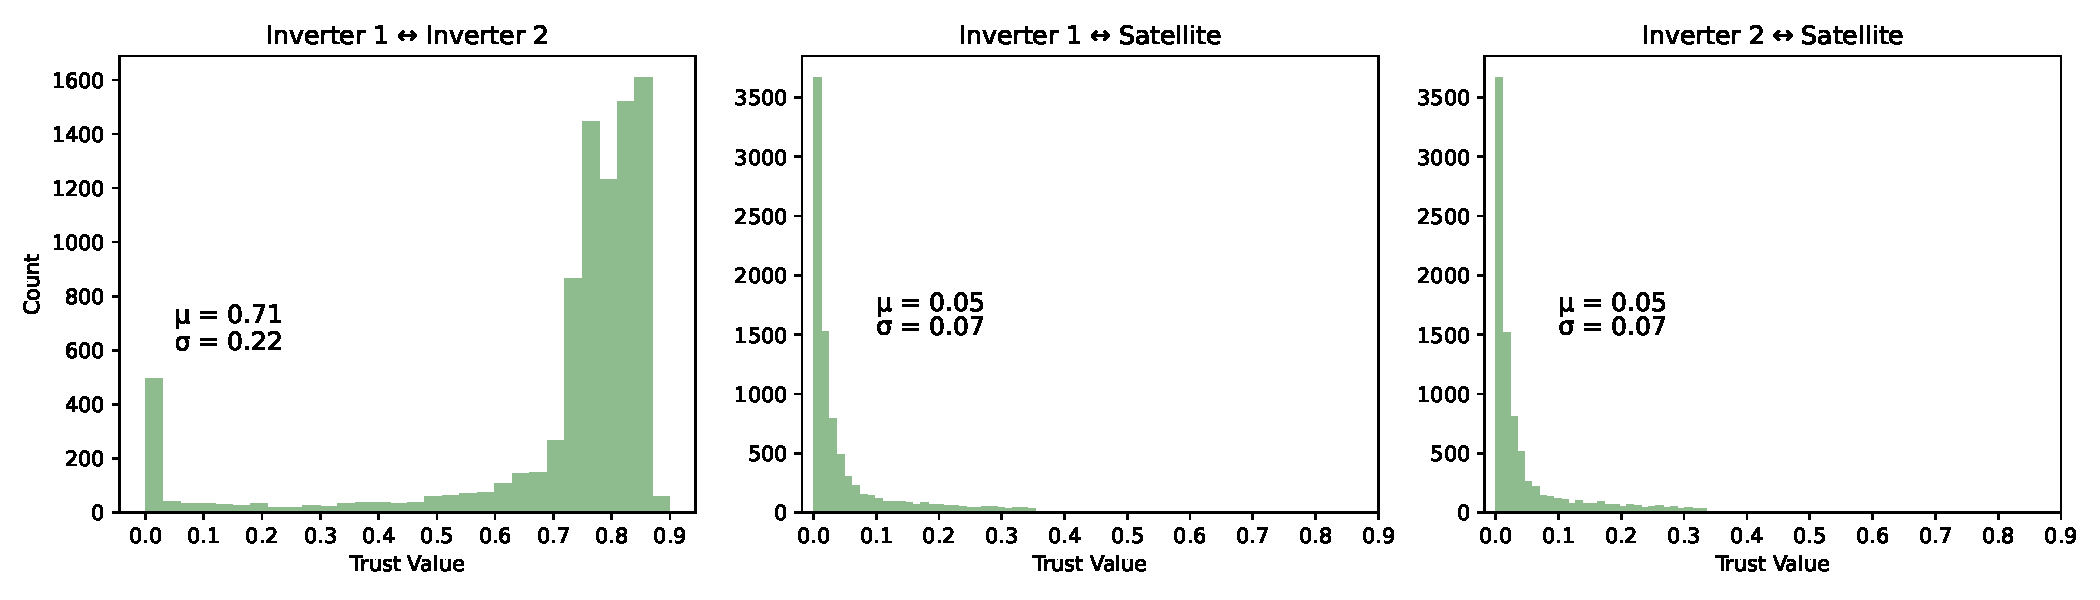
\includegraphics[width=\textwidth]{figures/chapter5/results/real/50_hist_trust_cells.pdf}
    \caption{Cells' trust measurement histogram.}
    \label{fig:cell_trust_hist}
\end{figure}

Analyzing the variables' trust indicators in figure \ref{fig:var_trust_hist} lets us confirm the strong relationship between AC power and DC side current. The DC side voltage trust presents a region of lower values apart from the highest frequency bin. These instances relate to the DC voltage behavior during sunrise and sunset, which was already flagged in section \ref{subsubsec:simnoanom}.

\begin{figure}[h!]
    \centering
    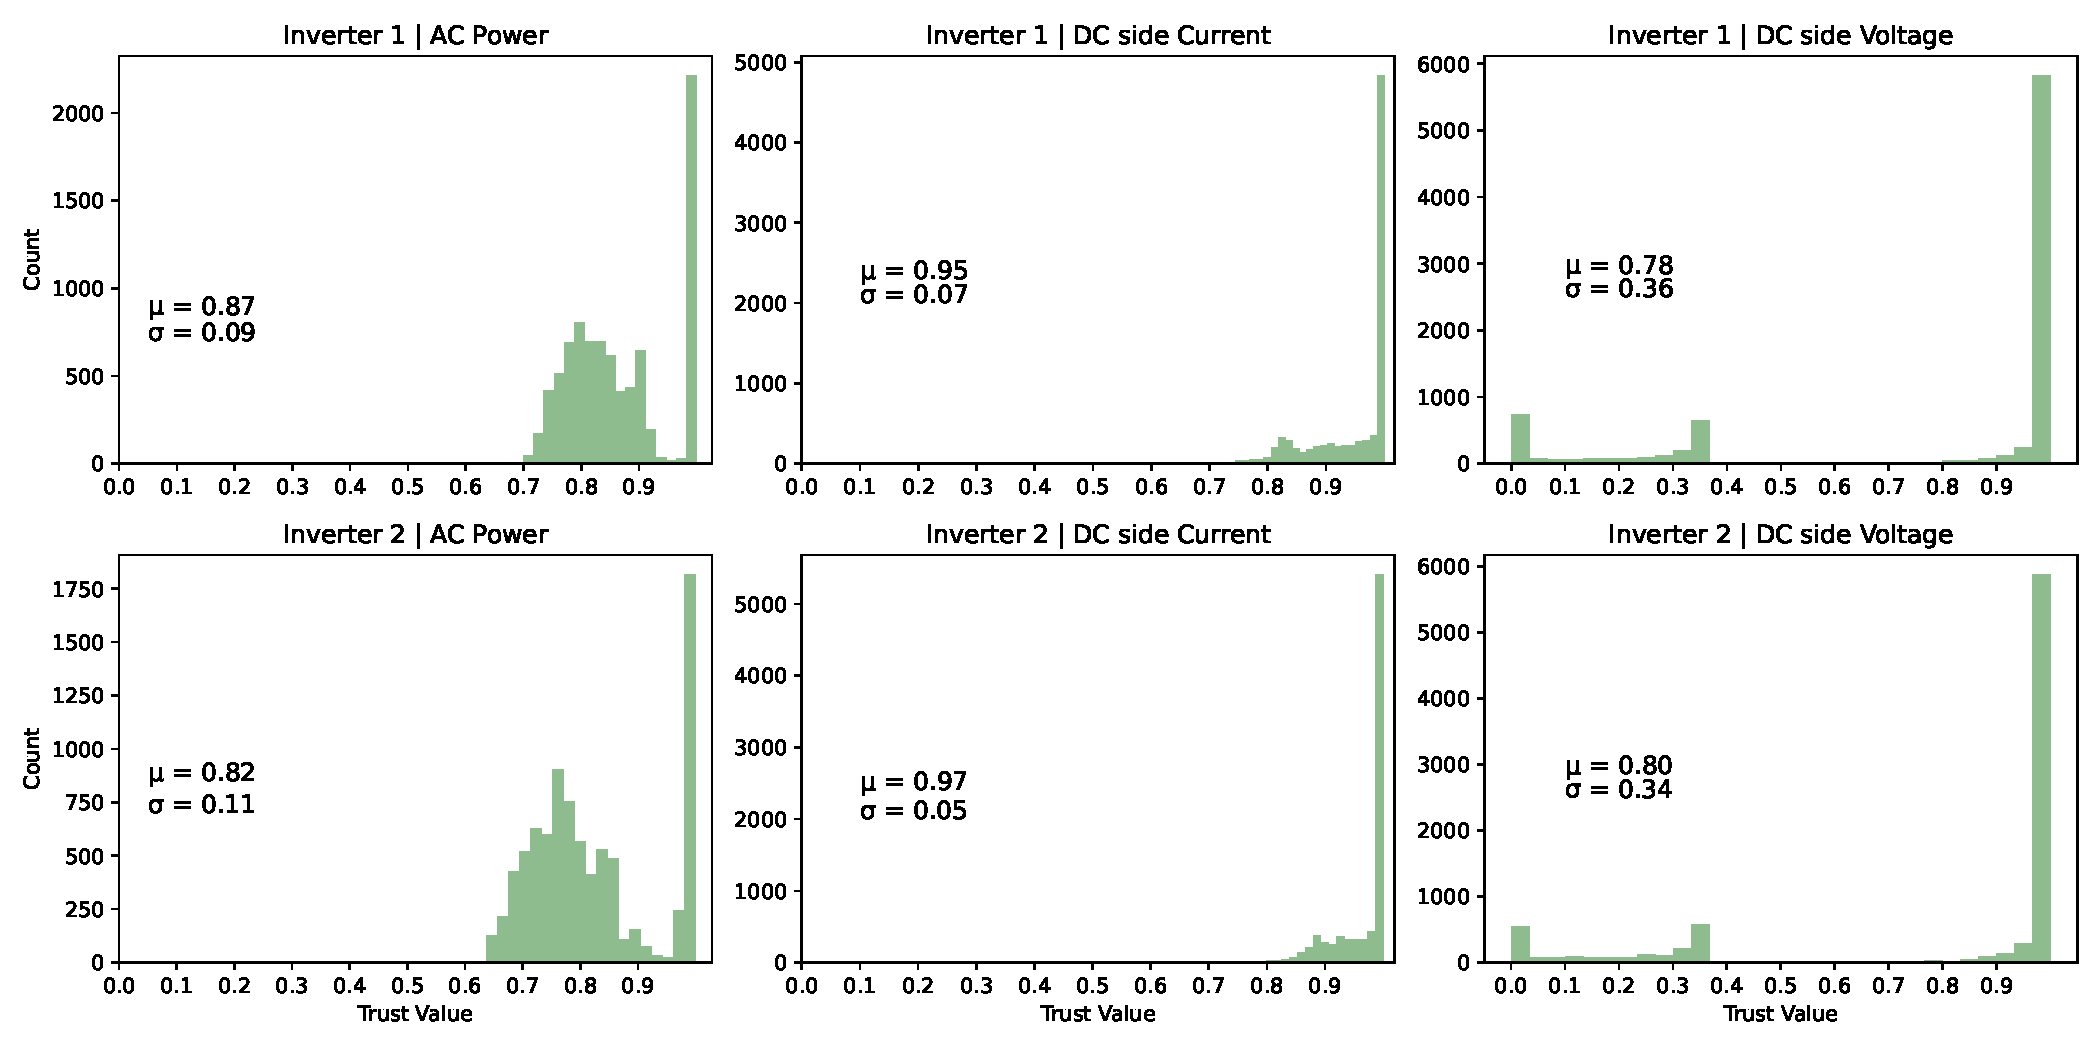
\includegraphics[width=\textwidth]{figures/chapter5/results/real/51_hist_trust_vars.pdf}
    \caption{Cell variables' trust measurement histogram.}
    \label{fig:var_trust_hist}
\end{figure}

Based on the information presented in figures \ref{fig:cell_trust_hist} and \ref{fig:var_trust_hist}, we can conclude that the inverter cell trust indicator is the most valuable feature of CellTAN for our particular network scenario. This indicator will be one of the primary analysis topics in the upcoming sections.

\subsubsection{Inverter Underperformance Detection}

The PV plugin successfully identified situations of underperformance when DC side measurements fell in the mapped region (figure \ref{fig:anomaly_decision_boundary}). Figure \ref{fig:plugin_detections} represents all the flagged samples from test data. The reason for missing samples closer to the column of typical MPPT operation is that we added a 5\% tolerance for identifying these situations. We considered this tolerance because alarming all underperformance situations would overwhelm the PV farm owner of non-severe and temporary cases. Regardless, the owner parametrizes this threshold when setting up the CellTAN.

\begin{figure}[h!]
    \centering
    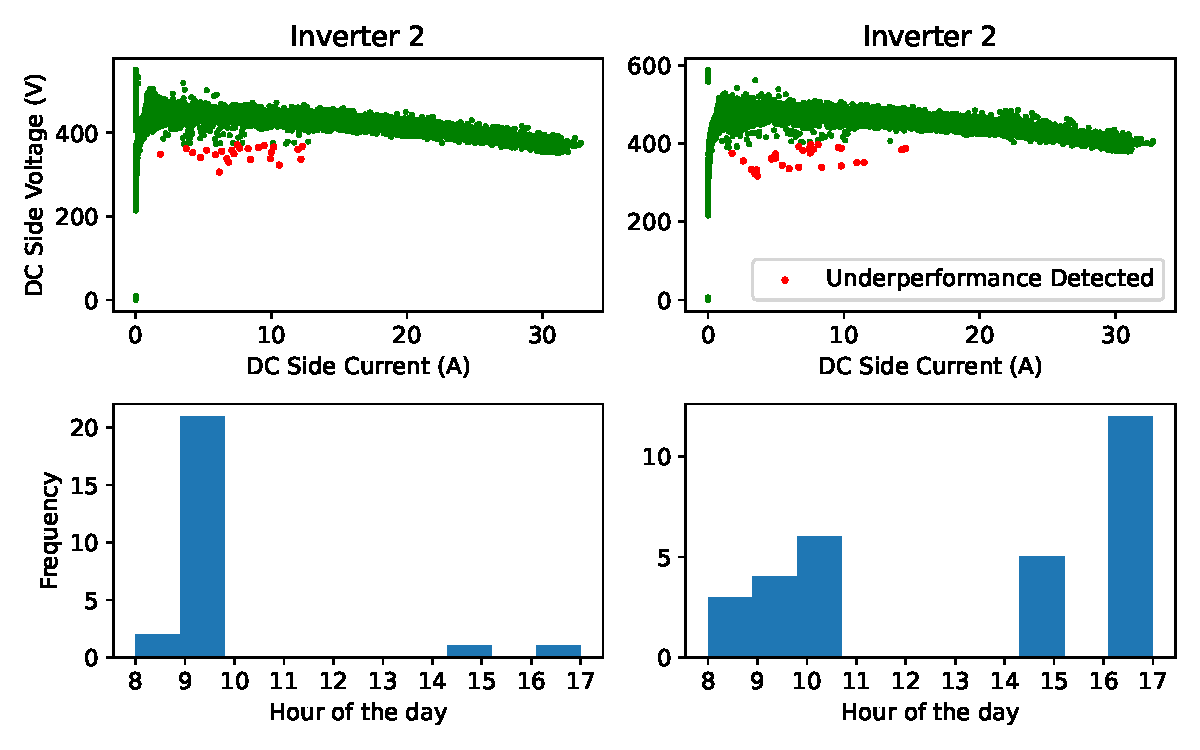
\includegraphics[width=0.9\textwidth]{figures/chapter5/results/real/53_pv_plugin_detections.pdf}
    \caption{I-V scatter of test data (both inverters) with detected underperformance instances colored red (top) and histogram based on the hour of detection (bottom).}
    \label{fig:plugin_detections}
\end{figure}

With the histogram in figure \ref{fig:plugin_detections}, we can assess that underperformance mostly happens during sunrise and sunset. The underperformance behavior affects inverter cells' trust, which reflects in this measurement dropping a lot during sunrise and sunset hours. Appendix \ref{ap3:alltimeseries} presents all the days with underperformance detections.

% \FloatBarrier
\subsubsection{Day-by-day analysis}

Reviewing the time series data of inverter AC power and trust between cells made us notice recurring patterns and situations throughout the test data. Figure \ref{fig:interesting_days} showcases the three main categories of days that stood out in the trust measurement profile. Looking at the bottom two AC power scatters, we can identify outlier regions reviewed from figure \ref{fig:real_sim_trust_scatter}. To satisfy the curiosity of observing the inverter cells' trust profile throughout the test dataset, we made it available in appendix \ref{ap3:alltimeseries}.

\begin{figure}[h!]
    \centering
    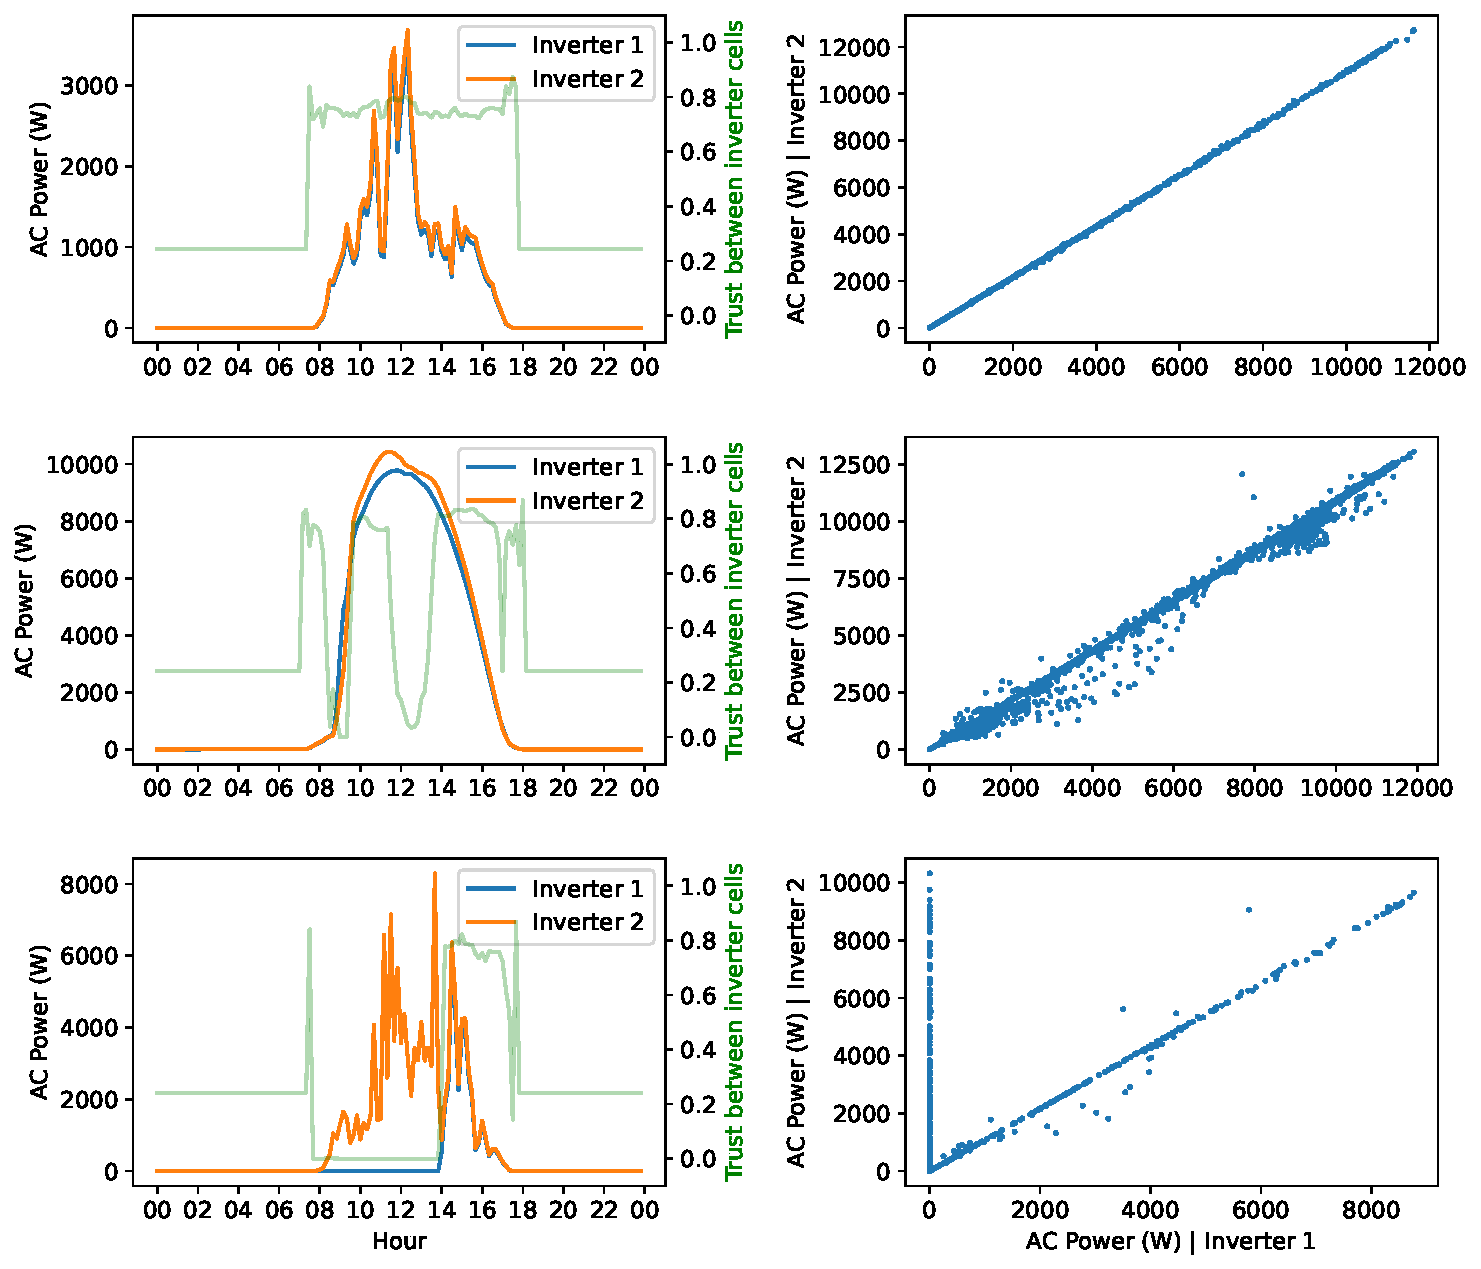
\includegraphics[width=0.9\textwidth]{figures/chapter5/results/real/type_of_days.pdf}
    \caption{Example days of inverters' highly correlated power (top), power mismatches (middle), and inverter one inoperational (bottom).}
    \label{fig:interesting_days}
\end{figure}

Figure \ref{fig:interesting_days_freq} showcases the frequency of each trust-based category. We can conclude that mild mismatches were very common, with a significantly larger frequency than the days of correlated production. The "Other" label refers to situations with slight power mismatches or voltage variations that change the trust measure enough not to be characterized as a highly correlated or power mismatch day.
The percentage of days where inverter one is not operating occurs when it either turns on after the beginning of sun hours (which happens most often) or remains off for the entire day (which only happened on January 8th, 2023).

There are nineteen days where the inverters demonstrate production profiles highly correlated throughout their daily cycle. Curiously, this only happens on cloudy days, making us question if their exposure to direct irradiance slightly varies due to different shading obstructions. We can see no outliers when checking out the I-V scatter for these days, which helps confirm the high trust value and no underperformance detections from the plugin.

On the eighty four days we found significant power mismatches, the most recurring pattern is sunrise-sunset and midday trust value dropping (between the two inverter cells). Analyzing the I-V variables shows that some samples lie in the underperformance region during these periods. The PV plugin detects most underperformance cases on these days, mainly in the morning and evening, as seen in figure \ref{fig:plugin_detections}. Inverter two dropping performance during peak sun hours could happen due to partial shading, inverter losses, or even string faults. It is helpful that the tool can identify these nuanced situations because it can assist technical teams in diagnosing the issue and preventing it from worsening if it stems from a fault.

On nine days, we found that inverter one did not produce energy during some sun hours (eight days) or was completely off (one day). There could be different reasons for this problem, but we would need labeled data to determine if it was equipment faults or planned maintenance shutdowns. This lack of identification is why this work does not present any classification steps besides the broad underperformance detection.

\begin{figure}[h!]
    \centering
    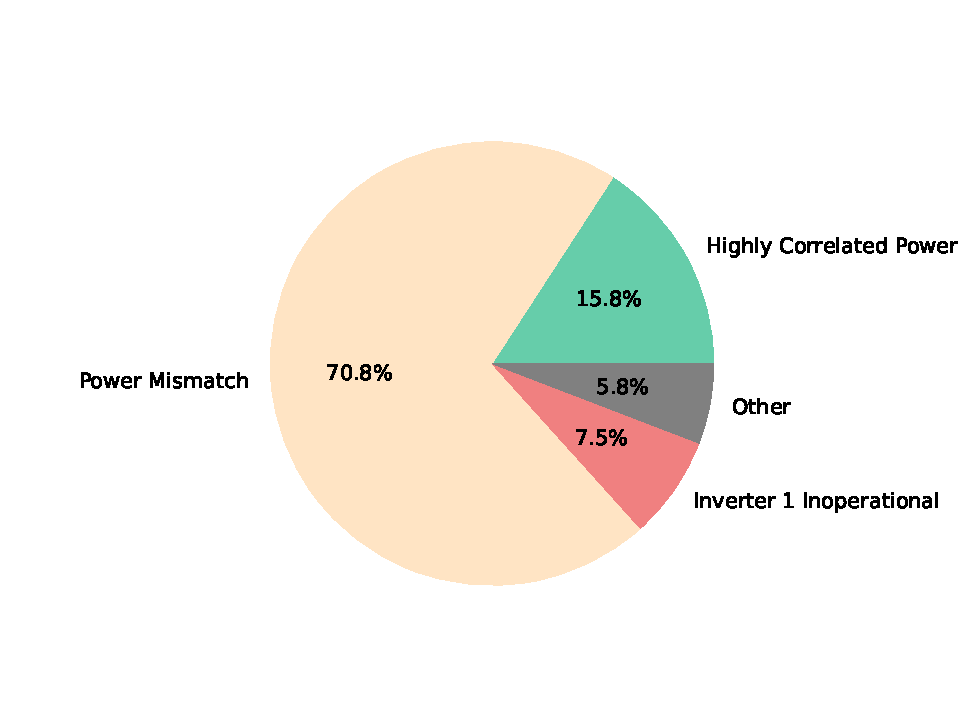
\includegraphics[width=0.75\textwidth,trim={0cm 2cm 0cm 2cm},clip]{figures/chapter5/results/real/situations_freq_pie.pdf}
    \caption{Frequency of days with identified scenarios based on trust measurement.}
    \label{fig:interesting_days_freq}
\end{figure}

The cell trust measurement's high variability is noticeable in figure \ref{fig:interesting_days}. When interpreting this value as a continuous signal, this characteristic supports the incorporation of moving average analysis for deciding anomaly occurrence. For example, if we configure the inverter cells to use a time bin as small as 10 minutes and a threshold of 0.2, the cell would flag anomalies for all the mismatches shown in \ref{fig:interesting_days} (middle). However, if we raise the window to a couple of hours, only the scenarios of inverter one inoperational would be identified. 
We can also verify the constant value displayed during nighttime. It is low because the cells find many night instances on their knowledge base when receiving related inputs. Increasing the total activation time decreases the trust measure (see \ref{subsec:trust}).

%todo mostrar moving averages?

% \FloatBarrier
\subsubsection{Using Contaminated Knowledge Base}


So far, all the results come from a CellTAN whose cells have a clean knowledge base. Undergoing the cleaning phase seemed the appropriate way to extract this tool's full potential, considering how its algorithms work. However, what if we do not clean the knowledge base? Furthermore, what if, in an actual application, that task is too time-consuming or challenging due to the volume of data or other issues?
Following this interest, we simulate the same test data with the same CellTAN configuration, changing the knowledge base for the original raw version. This dataset had various outliers in different regions, although its contamination was not overwhelming compared to the number of samples for regular operation.


\begin{figure}[h!]
    \centering
    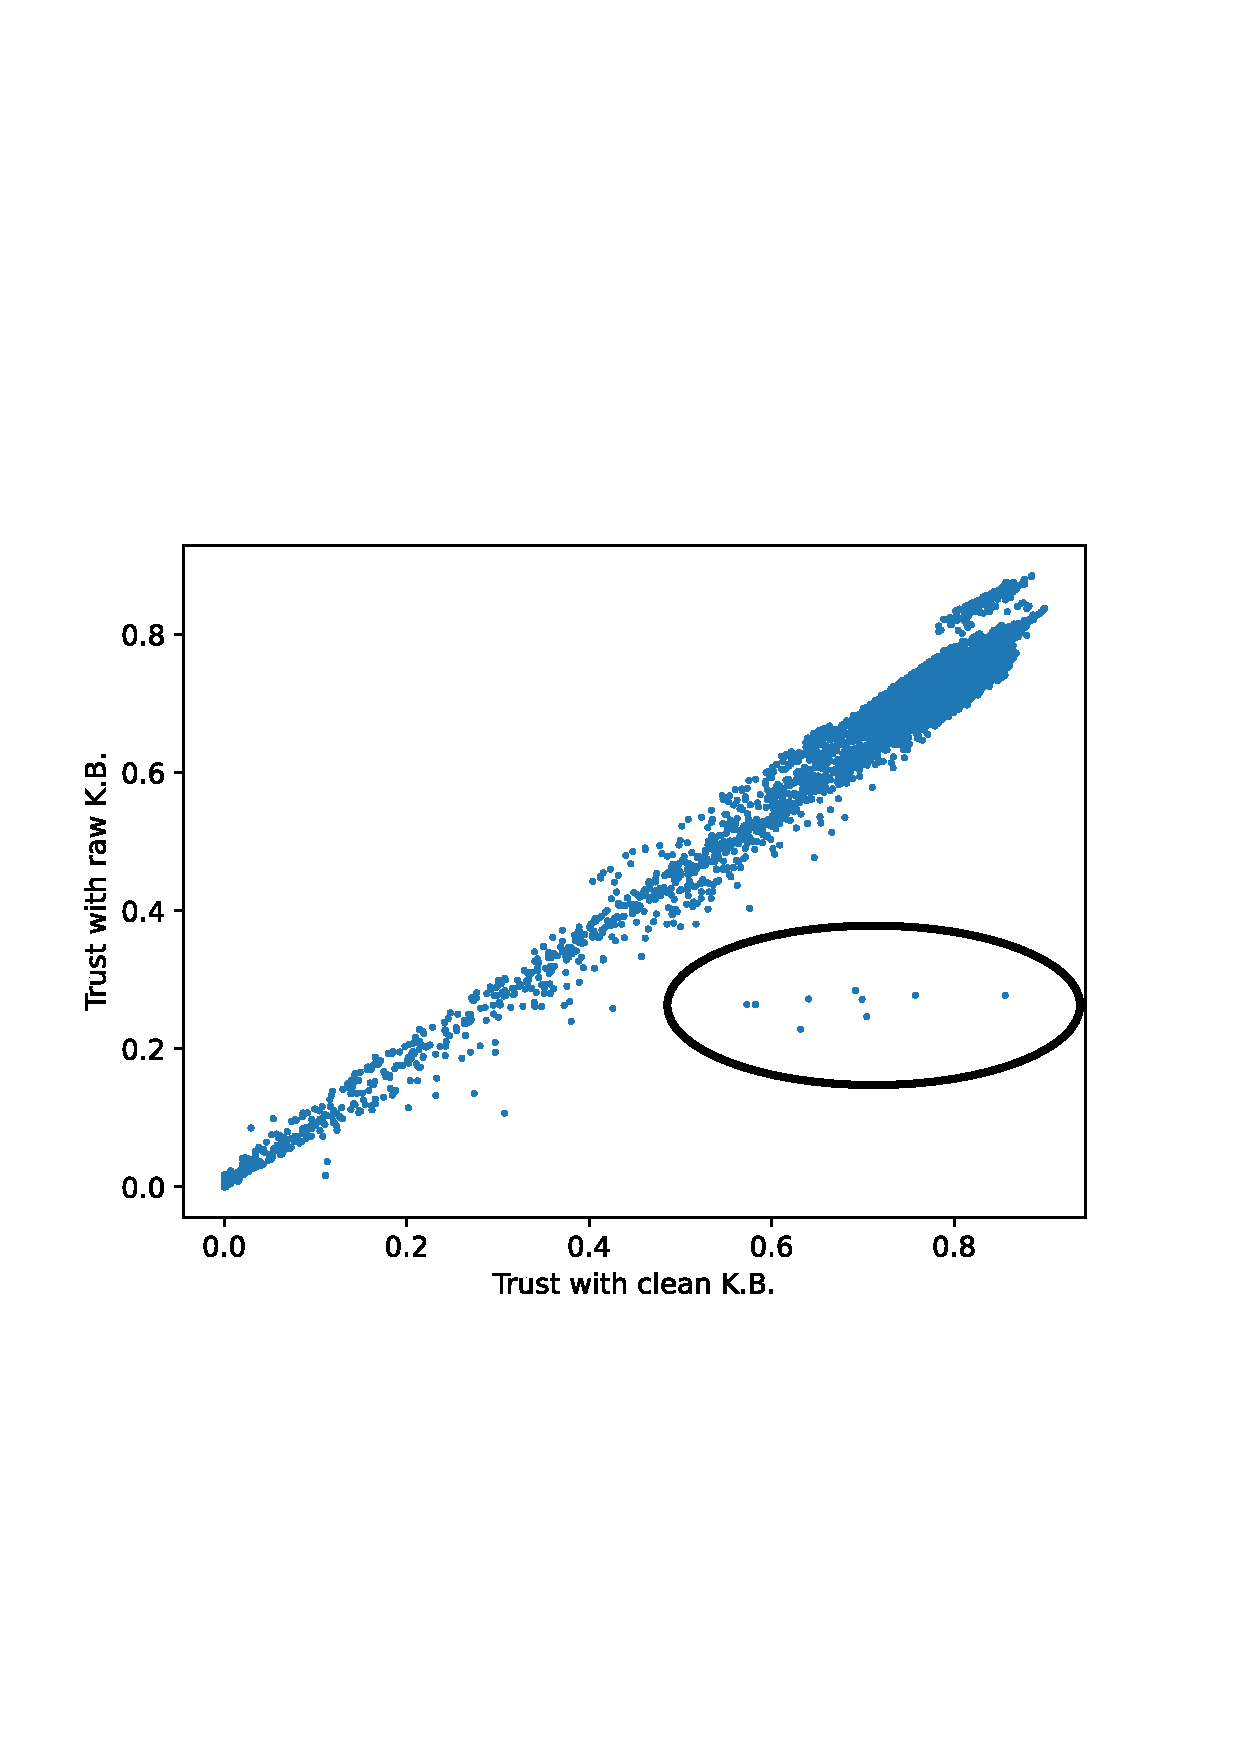
\includegraphics[width=0.6\textwidth,trim={0cm 7.5cm 0cm 9cm},clip]{figures/chapter5/results/real/trust_dirty_scatter_annotated.pdf}
    \caption{Scatter of trust measurements between inverter cells, with and without a clean knowledge base.}
    \label{fig:dirty_scatter}
\end{figure}

To our surprise, the trust indicator between the two inverter cells barely changed its behavior, confirmed by the scatter of the two in figure \ref{fig:dirty_scatter}. Still, there were some deviations, with the new trust measure being lower than the previous (on average) and some samples straying from the main trend line (contained in the black ellipse). We could identify these outlier instances alongside a very peculiar behavior by filtering the occurrences where the deviation was more than 0.2. What had happened was that both inverters shut off during sun hours on the days when these deviations occurred. The trust measurement with the clean knowledge base did not detect this anomaly, but it was very noticeable with the contaminated version.

\begin{figure}[h!]
    \centering
    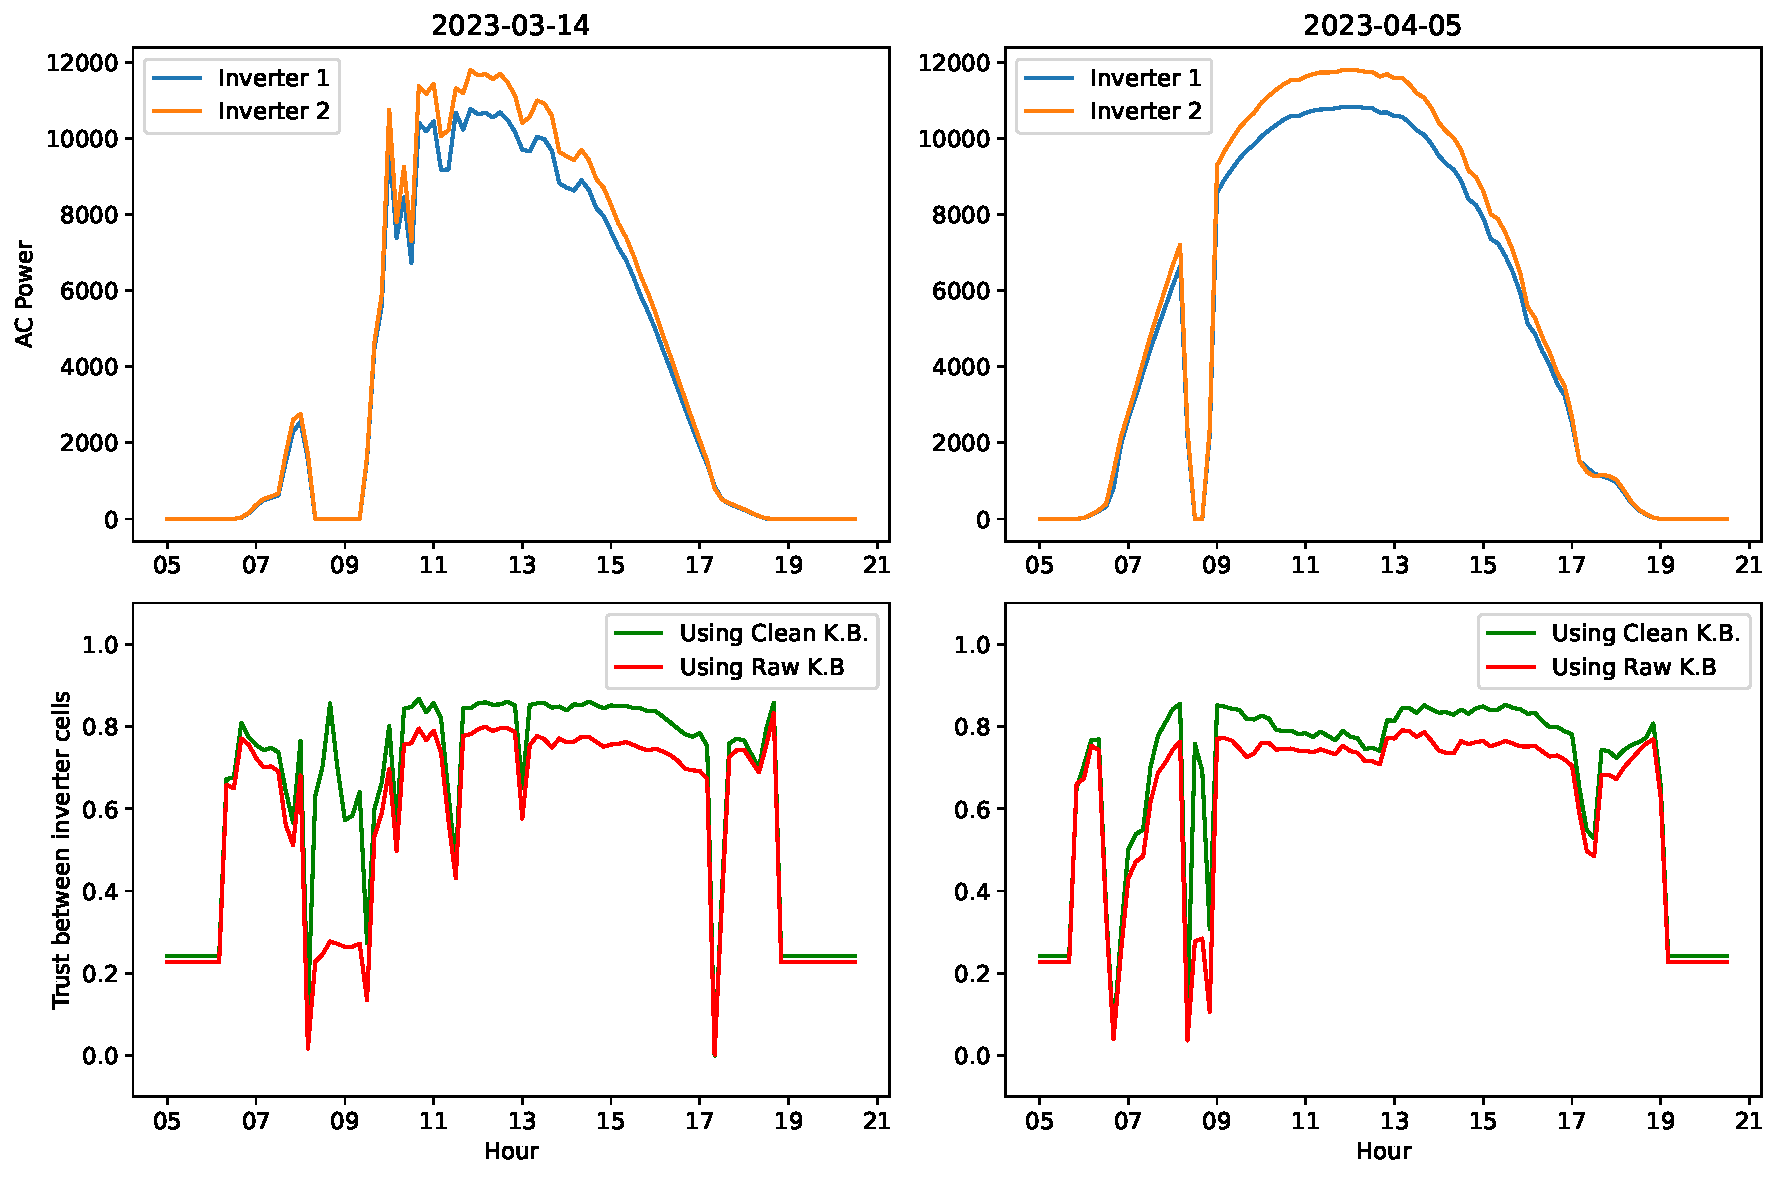
\includegraphics[width=0.8\textwidth]{figures/chapter5/results/real/trust_dirty_interesting_days.pdf}
    \caption{Days when the difference between trust of inverter cells with and without knowledge base is greater than 0.2.}
    \label{fig:dirty_interesting}
\end{figure}

% \subsection{Scaling Up}

% \dots

% \begin{figure}[h!]
%     \centering
%     \includegraphics[width=\linewidth]{figures/chapter4/cell/celltan.pdf}
%     \caption{Ilustrative overview of a CellTAN.}
%     \label{fig:celltan}
% \end{figure}

% Figure \ref{fig:celltan} illustrates a simple CellTAN network overview. Regarding the \textbf{Hub}, one might infer (correctly) that a central component breaks the non-centralized paradigm. Nevertheless, it is present to solve some real-life implementation challenges and limitations, as will be further discussed in this chapter.
